
\section{BÀI TẬP CUỐI CHƯƠNG 10}
\subsection{Câu hỏi trắc nghiệm}
\Opensolutionfile{ans}[ans/ans-9C10-OTC]
\begin{ex}%[Dự án EX-9-Đề Cương Toán 9]%[Hoàng Thanh Phương]%[9H4N1-3] 
	Thể tích của khối trụ có bán kính đáy $r$ và chiều cao $h$ bằng
	\choice
	{$\dfrac{1}{3}\pi r^2h$}
	{$2\pi rh$}
	{$\dfrac{4}{3}\pi r^2h$}
	{\True $\pi r^2h$}
	\loigiai{
		Công thức tính thể tích khối trụ có bán kính đáy $r$ và chiều cao $h$ là $V=\pi r^2h$.}
\end{ex}
\begin{ex}%[Dự án EX-9-Đề Cương Toán 9]%[Hoàng Thanh Phương]%[9H4N2-1]
	Công thức tính diện tích toàn phần hình nón có chiều cao $h$, bán kính đáy $r$ và đường sinh $l$ là
	\choice
	{$S_{tp}=\pi rl$}
	{$S_{tp}=\pi rl+2\pi r^2$}
	{$S_{tp}=2\pi rh+2\pi r^2$}
	{\True $S_{tp}=\pi rl+\pi r^2$}
	\loigiai{
		Theo công thức ta có $S_{tp}=\pi rl+\pi r^2$.	
	}
\end{ex}
\begin{ex}%[Dự án EX-9-Đề Cương Toán 9]%[Hoàng Thanh Phương]%[9H4N2-3] 
	Cho khối  nón có bán kính đáy $r=2$, chiều cao $h =5$. Tính thể tích $V$ của khối nón đó.
	\choice
	{$V=10\pi$}
	{$V=20\pi$}
	{\True $V=\dfrac{20\pi}{3}$}
	{$V=\dfrac{10\pi}{3}$}
	\loigiai{ \immini{
			Ta có $V = \dfrac{1}{3}\pi r^2 h =\dfrac{20\pi}{3}.$}{
			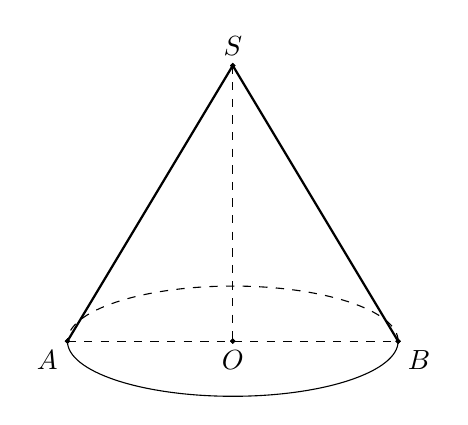
\begin{tikzpicture}[scale=0.7]
				\def\a{3} % bán trục lớn = bán kính trụ
				\def\b{1} % bán trục nhỏ
				\def\h{5} % chiều cao trụ
				\coordinate [label={below right}:$B$] (B) at (\a,0);
				\coordinate [label={below left}:$A$] (A) at (-\a,0);
				\coordinate [label={below}:$O$] (O) at (0,0);
				\coordinate [label={above}:$S$] (S) at (0,\h);
				\draw(S) circle (1pt) ;
				\draw(B) circle (1pt) ;
				\draw(A) circle (1pt) ;
				\draw(O) circle (1pt) ;
				\draw[thick]  (S)--(A);
				\draw[thick]  (S)--(B);
				\draw [dashed](A)--(B);
				\draw [dashed](S)--(O);
				\draw[dashed] (\a,0) arc [x radius=\a, y radius=\b, start angle=0, end angle=180];
				\draw(-\a,0) arc [x radius=\a, y radius=\b, start angle=180, end angle=360];
				\draw[fill](S) circle (1pt) ;
				\draw[fill](B) circle (1pt) ;
				\draw[fill](O) circle (1pt) ;
				\draw[fill](A) circle (1pt) ;
		\end{tikzpicture}}
	}
\end{ex}
\begin{ex}%[Dự án EX-9-Đề Cương Toán 9]%[Hoàng Thanh Phương]%[9H4N1-3] 
	Cho hình trụ có bán kính đáy bằng $4$, diện tích xung quanh bằng $48\pi$. Thể tích của khối trụ bằng
	\choice
	{$24\pi$}
	{\True $96\pi$}
	{$32\pi$}
	{$72\pi$}
	\loigiai{ Gọi hình trụ có bán kính và chiều cao lần lượt là $R$, $h$.\\
		Theo giả thiết $R=4$ và $S_{xq}=2\pi \cdot R\cdot h=48\pi$ nên $h=6$.\\ Do đó thể tích khối trụ $V=\pi \cdot R^2\cdot h=96\pi$.}
\end{ex} 
\begin{ex}%[Dự án EX-9-Đề Cương Toán 9]%[Hoàng Thanh Phương]%[9H4N3-3] 
	Thể tích của khối cầu có bán kính $R=4$ là
	\choice
	{\True $\dfrac{256\pi}{3}$}
	{$\dfrac{256}{3}$}
	{$64\pi$}
	{$\dfrac{64\pi}{3}$}
	\loigiai{
		$V=\dfrac{4}{3}\pi R^3=\dfrac{256}{3}\pi$.
	}
\end{ex}
\begin{ex}%[Dự án EX-9-Đề Cương Toán 9]%[Hoàng Thanh Phương]%[9H4H1-4] 
	Một công xưởng sản xuất $1000$ chiếc thùng bằng tôn không nắp, có đường kính đáy bằng $60$ cm và chiều cao bằng $90$ cm. Hỏi công xưởng cần phải chi ra bao nhiêu tiền mua nguyên liệu sản xuất, biết rằng tôn có giá $120\,000$ đồng/m$^2$ và hao hụt trong quá trình sản xuất là không đáng kể? (Lấy $\pi\approx 3{,}14$).
	\choice
	{$124\,344\,000$ đồng}
	{$316\,512\,000$ đồng}
	{\True $237\,384\,000$ đồng}
	{$252\,384\,000$ đồng}
	\loigiai{
		Diện tích tôn làm một thùng (không nắp) là $S=2\pi rh+\pi r^2=2\pi\cdot 0{,}3\cdot 0{,}9+\pi\cdot 0{,}3^2=1{,}9782$ m$^2$. \\
		Vậy diện tích tôn làm $1000$ thùng là $1978{,}2$ m$^2$. \\
		Tiền mua vật liệu là $237\,384\,000$ triệu đồng
	}
\end{ex}
\begin{ex}%[Dự án EX-9-Đề Cương Toán 9]%[Hoàng Thanh Phương]%[9H4N1-3] 
	Thể tích khối trụ sinh ra khi quay hình chữ nhật $ABCD$ quanh cạnh $AB$ biết $ AB=3$, $AD=4$ là
	\choice
	{\True $ V=48\pi$}
	{$V=36\pi$}
	{$V=24\pi$}
	{$V=18\pi$}
	\loigiai{
		\immini{
			Ta có $ r=BC=4, h=AB=3$. \\
			Suy ra $V=\pi r^2 h=\pi \cdot 4^2\cdot 3=48\pi$.
		}
		{
			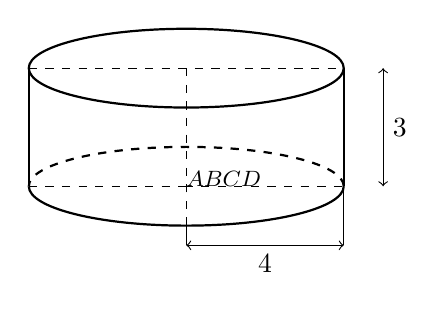
\begin{tikzpicture}[scale=0.5]
				\def\a{4} % bán trục lớn = bán kính trụ
				\def\b{1} % bán trục nhỏ
				\def\h{3} % chiều cao trụ
				% các chú thích
				\draw[<->, xshift=1cm] (\a,0)--(\a,\h) node[midway, right] {$3$};
				\draw[<->, yshift=-1.5cm] (0,0)--(\a,0) node[midway, below] {$4$};
				% vẽ các cạnh bên
				\draw[thick] (\a,0)--(\a,\h) (-\a,0)--(-\a,\h);
				\coordinate (C) at (\a,0);
				\coordinate (D) at (\a,\h);
				\coordinate (A) at (0,\h);
				\coordinate  (M) at (-\a,\h);
				\coordinate  (N) at (-\a,0);
				\coordinate (B) at (0,0);
				\draw [dashed] (M)--(D)--(C);
				\draw [dashed](A)--(B)--(C);
				\draw [dashed](N)--(B);
				\draw [dashed](0,-1.0)--(B);
				\draw  (\a,0)--(\a,-1.5);
				\draw  (0,-1)--(0,-1.5);
				% vẽ đáy dưới
				\draw[dashed, thick] (\a,0) arc [x radius=\a, y radius=\b, start angle=0, end angle=180];
				\draw[thick] (-\a,0) arc [x radius=\a, y radius=\b, start angle=180, end angle=360];
				% vẽ đáy trên
				\draw[thick] (0,\h) ellipse (\a cm and \b cm);
				% gán nhãn
				\tkzLabelPoint[above right](A){\footnotesize $A$}
				\tkzLabelPoint[above right](B){\footnotesize $B$}
				\tkzLabelPoint[right](C){\footnotesize $C$}
				\tkzLabelPoint[right](D){\footnotesize $D$}
				\tkzDrawPoints(A, B, C, D)
			\end{tikzpicture}
		}
	}
\end{ex}
\begin{ex}%[Dự án EX-9-Đề Cương Toán 9]%[Hoàng Thanh Phương]%[9H4H1-3] 
	\immini{Người ta cần sản xuất một chiếc cốc thủy tinh có dạng hình trụ không có nắp với đáy cốc và thành cốc làm bằng thủy tinh đặc, phần đáy cốc dày đều $1,5 \, cm$ và thành xung quanh cốc dày đều $0,2$ cm (hình vẽ). Biết rằng chiều cao của chiếc cốc là $15$ cm và khi đổ $180$ ml nước vào cốc thì đầy cốc. Tính thể tích thủy tinh cần làm chiếc cốc trên? (đơn vị cm$^3$, làm tròn đến hàng phần mười)}
	{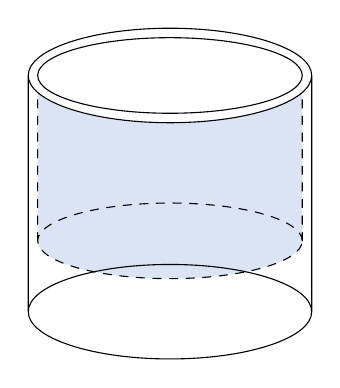
\begin{tikzpicture}[line join = round, line cap=round,>=stealth,font=\footnotesize,scale=0.6]
			\fill [line width=1.5pt,dashed,cyan!50!blue!20,opacity=0.7]
			(-2.8,1.5)--(-2.8,4.66)--(2.8,4.66)--(2.8,1.5)--cycle	
			(-2.8,1.5) arc (180:360:{2.8} and {0.8});
			;
			\draw[dashed]
			(0,1.5) ellipse ({2.8} and {0.8})
			(-2.8,1.5)--(-2.8,4.66)
			(2.8,1.5)--(2.8,4.66)
			;
			\fill[white]
			(0,5) ellipse ({3} and {1})
			;
			\draw
			(-3,0)--(-3,5)
			(3,0)--(3,5)
			(0,0) ellipse ({3} and {1})
			(0,5) ellipse ({3} and {1})
			(0,5) ellipse ({2.8} and {0.8})
			;
			
		\end{tikzpicture}	
	}
	\choice
	{$60{,}5$}
	{\True $60{,}7$}
	{$60{,}6$}
	{$60{,}8$}
	\loigiai
	{
			Thể tích phần chứa nước của cốc là $V=(r - 0{,}2)^2 (15 - 1{,}5) \pi$. \\
			Ta có: 
			$$ (r-0{,}2)^2 (15 - 1{,}5) \pi = 180\Rightarrow r = 0{,}2 + \sqrt{\dfrac{40}{3\pi}}.$$
			Thể tích thủy tinh cần là
			$$\pi \cdot \left(0{,}2 + \sqrt{\dfrac{40}{3\pi}} \right)^2 \cdot 15 - 180 = 60{,}7 \, (\text{cm}^3).$$
	}
\end{ex} 
\begin{ex}%[Dự án EX-9-Đề Cương Toán 9]%[Hoàng Thanh Phương]%[9H4H1-4] 
	Một em bé có một chiếc lọ chứa nước hình trụ không nắp, có bán kính đáy $5$ cm và chiều cao $20$ cm. Ban đầu, mực nước trong chiếc lọ bằng $\dfrac{9}{10}$ chiều cao của lọ nước. Em bé muốn thả một số viên bi có bán kính $0{,}5$ cm vào lọ nước để trang trí và nhận thấy rằng, khi thả tới viên bi thứ $x$ thì nước tràn ra ngoài. Giá trị của $x$ bằng bao nhiêu?
	\choice
	{$299$}
	{$300$}
	{\True $301$}
	{$302$}
	\loigiai{
		Lúc đầu mực nước trong bình là $18$ cm, do đó thể tích không gian còn trống trong lọ là $\pi \cdot 5^2\cdot 2=50\pi$ (cm$^3$). \\
		Thể tích một viên bi là $\dfrac{4}{3}\pi \cdot (0{,}5)^3=\dfrac{\pi}{6}$ (cm$^3$).  \\
		Ta có $50\pi:\dfrac{\pi}{6}=300$, vậy khi thả tới viên bi thứ $301$ thì nước sẽ bị tràn ra ngoài.\\
		 Vậy $x=301$.
	}
\end{ex}
\begin{ex}%[Dự án EX-9-Đề Cương Toán 9]%[Hoàng Thanh Phương]%[9H4H2-3] 
	Cho tam giác $AOB$ vuông tại $O$, $OA=4a$, $OB=3a$. Quay tam giác $AOB$ xung quanh cạnh $AB$ ta được một khối nón. Tính thể tích của khối nón này.
	\choice
	{\True $9{,}6\pi a^3$}
	{$10\pi a^3$}
	{$8{,}4\pi a^3$}
	{$4\pi a^3$}
	\loigiai{
		\immini{
			Kẻ đường cao $OH$ của tam giác vuông $AOB$.\\
			Khi quay tam giác vuông $AOB$ xung quanh cạnh $AB$ ta thu được hai khối nón có đỉnh là $A$ và $B$.
			Thể tích khối tạo thành bằng tổng thể tích của 2 khối nón trên.}
		{
			\begin{tikzpicture}[scale=0.85]
				\def\a{2.2}
				\def\b{0.5}
				\path
				(-3.5,0) coordinate (A)
				(2,0) coordinate (B)
				(0,\a) coordinate (O)
				(0,-\a) coordinate (Q)
				(intersection of A--B and O--Q) coordinate (H);
				\draw[dashed] (O) arc (90:270:{\b} and {\a});
				\draw (Q) arc (-90:90:{\b} and {\a});
				\draw (A)--(O)--(B)--(Q)--cycle;
				\draw[dashed] (A)--(B) (O)--(Q);
				\foreach \x/\dinh/\y in {O/H/B,A/O/B} \draw ($(\dinh)!5pt!(\x)$)--($(\dinh)!5pt!(\x)+(\dinh)!5pt!(\y)-(\dinh)$)--($(\dinh)!5pt!(\y)$); 
				\foreach \x/\g in
				{A/180,B/0,O/90,H/135}
				\fill[black](\x) circle (1pt)
				($(\x)+(\g:3mm)$) node{$\x$};
				\fill[black] (Q) circle (1pt);
		\end{tikzpicture}}
		\noindent Vậy ta có: $V=V_1+V_2=\dfrac{1}{3}\pi r^2h_1+\dfrac{1}{3}\pi r^2h_2=\dfrac{1}{3}\pi r^2(h_1+h_2) =\dfrac{1}{3}\pi\cdot OH^2\cdot AB$.\\
		Áp dụng hệ thức lượng trong tam gác vuông $AOB$ ta có
		$$\dfrac{1}{OH^2}=\dfrac{1}{OA^2}+\dfrac{1}{OB^2}=\dfrac{25}{144a^2}\Rightarrow OH=\dfrac{12a}{5}.$$
		$AB=\sqrt{OA^2+OB^2}=5a$.\\
		Vậy thể tích khối cần tìm là $V=\dfrac{1}{3}\pi\cdot\left(\dfrac{12a}{5}\right)^2\cdot 5a=9{,}6\pi a^3$.
	}
\end{ex}
\begin{ex}%[Dự án EX-9-Đề Cương Toán 9]%[Hoàng Thanh Phương]%[9H4V2-3] 
	\immini{Một cốc thủy tinh hình nón có chiều cao $20$ cm. Người ta đổ  vào cốc thủy tinh một lượng nước sao cho chiều cao của lượng nước trong cốc bằng $ \dfrac{3}{4} $ chiều cao cốc thủy tinh, sau đó người ta bịt kín miệng cốc rồi lật úp cốc xuống như hình vẽ thì chiều cao của nước lúc này là bao nhiêu (làm tròn đến chữ số thập phân thứ 2).
		\choice
		{$2{,}21$ cm}
		{$5{,}09$ cm}
		{$4{,}27$ cm}
		{\True $3{,}34$ cm}}
	{\begin{tikzpicture}[>=stealth,line join=round,line cap=round,font=\footnotesize,scale=0.6]
			\coordinate (A) at (2,0);
			\coordinate (B) at (-2,0);
			\coordinate (S) at (0,-6);
			\coordinate (M) at ($(S)!3/4!(A)$);
			\fill[cyan!70!green] (S)--(M)arc(0:180:1.5 and 1/6)--cycle;
			\fill[cyan!30] (M)arc(0:180:1.5 and 1/6)arc(180:360:1.5 and 1/6);
			\draw (0,0)ellipse(2 and 2/3) (A)--(S)--(B) (M)arc(0:-180:1.5 and 1/6);
			\draw[dashed] (M)arc(0:180:1.5 and 1/6);
			\coordinate (A1) at (3,-5.63);
			\coordinate (B1) at (7,-5.63);
			\coordinate (S1) at (5,0.37);
			\coordinate (M1) at ($(A1)!1/10!(S1)$);
			\fill[cyan!70!green] (A1)--(M1)arc(180:0:9/5 and 3/5)--(B1)arc(0:-180:2 and 2/3);
			\fill[cyan!30] (M1)arc(180:0:9/5 and 3/5)arc(0:-180:9/5 and 3/5);
			\draw (A1)--(S1)--(B1)arc(0:-180:2 and 2/3) (M1)arc(-180:0:9/5 and 3/5);
			\draw[dashed] (M1)arc(180:0:9/5 and 3/5);
	\end{tikzpicture}}
	\loigiai{
		\immini{Gọi $r_1$, $h_1$, $V_1$ lần lượt là bán kính đáy, chiều cao và thể tích khối nón giới hạn bởi phần chứa nước lúc ban đầu; $r$, $h$, $V$ lần lượt là bán kính đáy, chiều cao và thể tích khối nón giới hạn bởi cốc thuỷ tinh; $h_2$ là chiều cao mực nước sau khi úp ngược cốc. Theo tính chất tam giác đồng dạng ta có $$\dfrac{r_1}{r}=\dfrac{h_1}{h}=\dfrac{3}{4}\Rightarrow \dfrac{V_1}{V}=\left(\dfrac{h_1}{h}\right)^3=\dfrac{27}{64}.$$
			Sau khi lộn ngược cốc, tỉ số thể tích giữa phần không gian trong cốc không chứa nước và thể tích cốc bằng
		}
		{\begin{tikzpicture}[>=stealth,line join=round,line cap=round,font=\footnotesize,scale=0.65]
				\coordinate (A) at (2,0);
				\coordinate (B) at (-2,0);
				\coordinate (S) at (0,-6);
				\coordinate (M) at ($(S)!3/4!(A)$);
				\fill[cyan!70!green] (S)--(M)arc(0:180:1.5 and 1/6)--cycle;
				\fill[cyan!30] (M)arc(0:180:1.5 and 1/6)arc(180:360:1.5 and 1/6);
				\draw (0,0)ellipse(2 and 2/3) (A)--(S)--(B) (M)arc(0:-180:1.5 and 1/6);
				\draw[dashed] (M)arc(0:180:1.5 and 1/6);
				\coordinate (A1) at (3,-5.63);
				\coordinate (B1) at (7,-5.63);
				\coordinate (S1) at (5,0.37);
				\coordinate (M1) at ($(A1)!1/10!(S1)$);
				\fill[cyan!70!green] (A1)--(M1)arc(180:0:9/5 and 3/5)--(B1)arc(0:-180:2 and 2/3);
				\fill[cyan!30] (M1)arc(180:0:9/5 and 3/5)arc(0:-180:9/5 and 3/5);
				\draw (A1)--(S1)--(B1)arc(0:-180:2 and 2/3) (M1)arc(-180:0:9/5 and 3/5);
				\draw[dashed] (M1)arc(180:0:9/5 and 3/5);
				\draw[<->] ($(A)+(.5,0)$)--+(-90:6)node[pos=.7,left]{$20$ cm};
				\draw[<->] ($(S)+(-2.3,0)$)--+(90:4.5)node[pos=.5,left]{$15$ cm};
		\end{tikzpicture}}
		$$1-\dfrac{27}{64}=\dfrac{(h-h_2)^3}{h^3}\Leftrightarrow\dfrac{37}{64}=\dfrac{(20-h_2)^3}{20^3}\Leftrightarrow 20-h_2=5\sqrt[3]{37}\Leftrightarrow h_2=20-5\sqrt[3]{7}\approx 3{,}34.$$
	}
\end{ex}
\begin{ex}%[Dự án EX-9-Đề Cương Toán 9]%[Hoàng Thanh Phương]%[9H4V3-4] 
	\immini{Để phòng tránh trẻ em bị đuối nước, người ta quyết định dùng đất để lấp một cái ao dạng nửa hình cầu, mặt ao hình tròn có đường kính $10$ m.
		Người ta tính thể tích nước trong ao theo m$^3$. Giả sử mực nước trong ao bằng với mặt đất xung quanh và các sinh vật, vật thể khác trong ao có thể tích không đáng kể. 
	}{
		\begin{tikzpicture}[line join = round, line cap=round,>=stealth,font=\footnotesize,scale=1]
			\def\r{1.5} \def\c{0.5} 
			\fill[pattern={crosshatch dots},pattern color=blue] (0,0)--++(0:\r) arc (0:-180:\r)--(0,0);
			\filldraw[pattern=horizontal lines] 
			(0,0)++(0:\r) arc (0:-180:\r)--++(180:\c)--++(0.1,-0.4)--++(-0.2,-0.7)--++(0.2,-0.6)--++(0:\r*2+0.8)--++(0.2,0.6)--++(-0.2,0.7)--++(0.1,0.4)--++(180:\c);
			\draw[<->] (-\r,0.2)--++(0:\r*2) node[midway,above]{$10$ m};
		\end{tikzpicture}
	}
	\immini{Người ta thuê những xe tải có thùng xe dạng hình hộp chữ nhật, lòng trong thùng dài $9{,}9$ m, rộng $2{,}37$ m và cao $0{,}85$ m. Nhưng con đường từ nơi cung cấp đất đến ao bị giới hạn trọng tải của phương tiện tham gia giao thông nên xe chỉ chở được $85\%$ thể tích của lòng trong thùng xe. Hỏi cần thuê ít nhất bao nhiêu xe để lấp đầy cái ao? (Đất chở trên xe được nén chặt và gần như không có khoảng trống trong khối đất).
	}{
		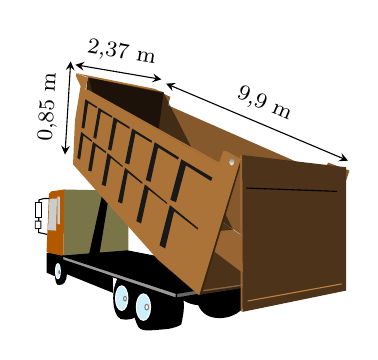
\begin{tikzpicture}[scale=0.6, font=\footnotesize, line join=round, line cap=round, >=stealth]
			%Gầm xe
			\fill[black](-1.53,-1.96) .. controls (-1.65,-2.27) and (-1.63,-2.54) .. (-1.47,-2.82) .. controls (-1.34,-2.85) and (-1.22,-2.83) .. (-1.17,-2.79) .. controls (-1.1,-2.95) and (-1.13,-3.09) .. (-0.8,-3.06) .. controls (-0.65,-3.05) and (-0.55,-3.04) .. (-0.45,-3.03) .. controls (-0.35,-3.01) and (-0.27,-2.99) .. (-0.18,-2.94) .. controls (-0.13,-2.7) and (-0.11,-2.58) .. (-0.13,-2.43) .. controls (-0.03,-2.49) and (0.07,-2.52) .. (0.18,-2.53) .. controls (0.26,-2.71) and (0.41,-2.82) .. (0.7,-2.8) .. controls (1.01,-2.77) and (1.23,-2.56) .. (1.26,-2.3) .. controls (1.17,-2.05) and (0.71,-2.05) .. (-0.15,-2.12) .. controls (-0.61,-2) and (-0.99,-1.94) .. (-1.38,-1.91);
			\fill[black](-2.87,-1.91) -- (-3.03,-1.84) -- (-3.03,-1.43) -- (-2.96,-1.42) -- (-2.65,-1.48) -- (-2.6,-1.75) -- (-2.84,-1.9);
			\fill[black](-2.65,-1.59) -- (-2.66,-1.85) -- (-1.62,-2.27) -- (-1.63,-1.93);
			%Đầu xe
			\fill[orange!70!black](-2.67,-1.49) -- (-3.03,-1.41) node (v3) {} -- (-2.98,-0.17) -- (-2.93,-0.12) -- (-2.66,-0.08)--cycle;
			\fill[yellow!40!black](-2.67,-1.49) -- (-1.3,-1.38) --  (-1.3,-0.11) -- (-2.66,-0.08)--cycle;
			\fill[gray!40] (-2.83,-0.95) -- (-3,-0.94) -- (-2.97,-0.28) -- (-2.81,-0.27)--cycle;
			\fill[gray!40] (-2.8,-0.23) -- (-2.75,-0.23) -- (-2.75,-0.82) -- (-2.8,-0.81);
			%Gương
			\draw (-2.98,-0.27) -- (-3.08,-0.27) -- (-3.19,-0.3) -- (-3.2,-0.99) -- (-3.02,-1.03);
			\fill[black] (-3.13,-0.34) -- (-3.28,-0.34) -- (-3.28,-0.68) -- (-3.13,-0.68);
			\fill[white] (-3.26,-0.36) -- (-3.15,-0.36) -- (-3.15,-0.66) -- (-3.26,-0.66);
			\fill[black]  (-3.28,-0.74) -- (-3.14,-0.74) -- (-3.14,-0.91) -- (-3.28,-0.92);
			\fill[white] (-3.26,-0.76) -- (-3.16,-0.76) -- (-3.16,-0.89) -- (-3.26,-0.9);
			%Bánh sau
			\fill[black] (-1.44,-2.38)  ellipse (0.18 and 0.44);
			\draw[white,fill=cyan!20]   (-1.44,-2.38)  ellipse (0.13 and 0.26);
			\draw  [gray,fill=white](-1.37,-2.39) ellipse (0.03 and 0.05);
			\fill[black] (-0.97,-2.58) ellipse (0.17 and 0.47);
			\draw[white,fill=cyan!20] (-0.98,-2.57) ellipse (0.15 and 0.28);
			\draw[gray,fill=white]  (-0.91,-2.57) ellipse (0.04 and 0.06);
			%Bánh trước
			\fill[black](-2.78,-2.1) .. controls (-2.73,-2.1) and (-2.67,-2.1) .. (-2.65,-2.05) .. controls (-2.59,-1.96) and (-2.58,-1.81) .. (-2.65,-1.67) .. controls (-2.7,-1.63) and (-2.76,-1.61) .. (-2.82,-1.63);
			\fill[black] (-2.79,-1.8) ellipse (0.07 and 0.3);
			\draw [white,fill=cyan!20]  (-2.79,-1.81) node (v4) {} ellipse (0.05 and 0.16);
			\draw  [gray,fill=white] (-2.76,-1.83) ellipse (0.01 and 0.03);
			%Sàn xe
			\draw [fill=black](-2.69,-1.49) -- (-0.28,-2.28) -- (1.67,-1.96) -- (-1.32,-1.38)--cycle;
			\draw [fill=black!40](-2.69,-1.49) node (v2) {} -- (-0.28,-2.28) -- (-0.29,-2.38) -- (-2.69,-1.57)--cycle;
			\draw [fill=black!60](-0.28,-2.38) -- (-0.28,-2.28) -- (1.67,-1.96) -- (1.67,-2.04)--cycle;
			%Pistong thủy lực
			\draw [fill=black](-2.13,-1.5) -- (-1.83,-0.14) -- (-1.72,-0.2) -- (-1.94,-1.55);
			%Thùng xe
			\fill[brown!70!black](-0.56,1.95) -- (-0.41,1.88) -- (-0.46,1.7) -- (2.82,0.26) --(2.93,0.49) -- (3.38,0.32)-- (2.59,-2.05) -- (-0.92,0.32)--cycle;
			\fill[brown!80!black](-2.32,0.47)  -- (0.31,-2.23) --(2.34,-1.9) -- (-0.92,0.32)--cycle;
			\fill[brown!30!black](-2.19,2.04) -- (-2.16,2.3) -- (-0.55,1.98) -- (-0.75,0.52);
			\fill[brown!90!black](-2.14,2.29) -- (-2.39,2.38) -- (-0.74,2.05) -- (-0.55,1.96);
			\fill[black,opacity=0.5](-0.56,1.98) -- (0.92,-0.93) -- (0.02,-1.02) -- (1.39,-2.05) node (v1) {} -- (0.27,-2.21) -- (-1.46,-0.36) -- (-2.14,2.29)--cycle;
			%Nắp đuôi
			\fill[brown!30!black](1.05,0.55) -- (0.2,-2.31) -- (1.16,-2.16) -- (1.21,-2.11) -- (0.27,-2.24) -- (1.11,0.55);
			\fill[brown!40!black](1.11,0.65) -- (3.31,0.39) -- (3.31,-2.22) -- (1.12,-2.67);
			\draw (1.2,-0.05) -- (3.11,-0.12);
			\draw [brown](1.23,-2.44) -- (3.21,-2.08);
			\fill[brown!80!black](1.11,0.65) -- (1.06,0.64) -- (1.08,-2.65) -- (1.12,-2.67);
			\fill[brown!90!black](-2.15,2.28) -- (-2.4,2.38) -- (-2.41,2.32) -- (-2.31,2.11) -- (-2.43,1.38) -- (-2.47,0.45) -- (-0.68,-1.56) -- (0.2,-2.32) -- (1.07,0.53) -- (0.71,0.73) -- (0.61,0.45) -- (-2.21,2.04);
			\fill[brown!90!black] (0.72,0.72) -- (0.76,0.74) -- (1.11,0.55) -- (1.06,0.54);
			\fill[brown!90!black](-2.19,2.02) -- (-2.15,2.03) -- (0.62,0.49) -- (0.62,0.45);
			%Thành thùng
			\fill[black!90](0.48,0.17) -- (-0.18,0.56) -- (-0.41,-0.3) -- (-0.29,-0.35) -- (-0.08,0.43) -- (0.45,0.1);
			\fill[black!90](-0.23,0.6) -- (-0.74,0.92) -- (-0.93,0.12) -- (-0.83,0.08) -- (-0.67,0.81) -- (-0.25,0.55);
			\fill[black!90](-0.8,0.95) -- (-1.22,1.21) -- (-1.37,0.48) -- (-1.28,0.45) -- (-1.15,1.11) -- (-0.81,0.91);
			\fill[black!90](-1.27,1.24) -- (-1.61,1.45) -- (-1.73,0.77) -- (-1.66,0.74) -- (-1.54,1.36) -- (-1.27,1.2);
			\fill[black!90](-1.64,1.47) -- (-1.93,1.65) -- (-2.04,1.02) -- (-1.98,0.99) -- (-1.88,1.57) -- (-1.65,1.44);
			\fill[black!90](-1.96,1.67) -- (-2.21,1.83) -- (-2.29,1.22) -- (-2.23,1.21) -- (-2.15,1.75) -- (-1.97,1.64);
			\fill[black!90](0.18,-0.9) -- (-0.42,-0.41) -- (-0.64,-1.26) -- (-0.52,-1.33) -- (-0.33,-0.54) -- (0.17,-0.93);
			\fill[black!90](-0.48,-0.36) -- (-0.95,0.03) -- (-1.13,-0.75) -- (-1.03,-0.8) -- (-0.87,-0.08) -- (-0.48,-0.39);
			\fill[black!90](-1,0.07) -- (-1.37,0.38) -- (-1.52,-0.34) -- (-1.43,-0.38) -- (-1.31,0.28) -- (-1.01,0.04);
			\fill[black!90](-1.42,0.42) -- (-1.74,0.69) -- (-1.86,0.02) -- (-1.78,-0.01) -- (-1.67,0.59) -- (-1.42,0.39);
			\fill[black!90](-1.77,0.72) -- (-2.05,0.93) -- (-2.15,0.32) -- (-2.08,0.3) -- (-1.99,0.84) -- (-1.78,0.69);
			\fill[black!90](-2.07,0.96) -- (-2.3,1.14) -- (-2.38,0.59) -- (-2.32,0.55) -- (-2.25,1.06) -- (-2.08,0.93);
			\shade[brown!90!black] (0.89,0.51) ellipse (0.05 and 0.08);
			%Kích thước
			\draw [<->](-0.5,2.16) --node[midway,above,sloped]{$9{,}9$ m} (3.35,0.53);
			\draw [<->](-0.6,2.25) --node[midway,above,sloped]{$2{,}37$ m} (-2.42,2.56);
			\draw [<->](-2.64,0.66) --node[midway,above,sloped]{$0{,}85$ m} (-2.52,2.63);
		\end{tikzpicture}		
	}
	\choice
	{$15$}
	{\True $16$}
	{$17$}
	{$18$}
	\loigiai{
		Bán kính của hình cầu là $R=\dfrac{1}{2}\cdot 10=5$ (m). \\
		Thể tích của ao có dạng nửa hình cầu là 
		$$V=\dfrac{1}{2}\cdot\dfrac{4}{3}\pi R^3=\dfrac{1}{2}\cdot\dfrac{4}{3}\cdot\pi\cdot 5^3=\dfrac{250\pi}{3}\approx 261{,}8~(\text{m}^3).$$
		Thể tích của thùng xe là 
		$$9{,}9\cdot 2{,}37\cdot 0{,}85 = 19{,}94355~(\text{m}^3).$$
		Vì xe chỉ chở được $85\%$ thùng xe nên thể tích đất chở được là 
		$$19{,}94355\cdot 85\%\approx 16{,}952~(\text{m}^3).$$
		Ta có $\dfrac{261{,}8}{16{,}952}\approx 15{,}44$, do đó cần thuê ít nhất $16$ xe mới có thể lấp đầy được ao đó.
	}
\end{ex}
\subsection{Bài tập tự luận}
\begin{bt}%[Dự án EX-9-Đề Cương Toán 9]%[Hoàng Thanh Phương]%[9H4H4-4]
	\immini{Một cốc nước hình trụ cao $12$ cm, đường kính $7$ cm, độ dày cốc $2$ mm, độ dày đáy là $5$ mm đang chứa $80$ ml nước. Người ta bỏ các viên đá hình lập phương cạnh $2$ cm vào cốc sao cho khi tan chảy hết thì mực nước sau cùng cách miệng cốc không vượt quá $1$ cm. Hỏi có thể bỏ tối đa được bao nhiêu viên đá như thế vào cốc?}
	{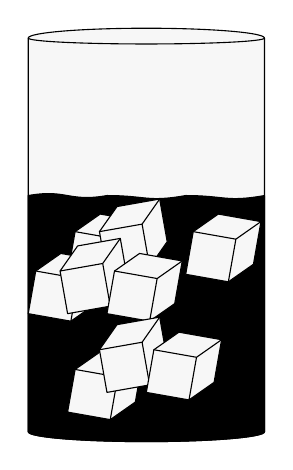
\begin{tikzpicture}[line join = round, line cap=round,>=stealth,font=\footnotesize,scale=.5]
			\draw[fill=black!3] (0,0) arc(180:360:3cm and 0.25cm) -- (6,10) arc(0:180:3cm and 0.25cm) -- cycle;
			\draw (0,10) arc(180:360:3cm and 0.15cm);
			\draw[fill=black] 
			(6,6) ..controls +(190:1) and +(0:1) .. (4,6) 
			..controls +(190:1) and +(0:1) .. (2,6) 
			..controls +(190:1) and +(10:1) .. (0,6) 
			-- (0,0) arc(180:360:3cm and 0.25cm) -- cycle;
			\tikzset{da/.pic={ 
					\draw[fill=black!3!white] (0,0) -- (1,0)--(1.5,0.5)--(1.5,1.5)--(0.5,1.5)--(0,1)--cycle;
					\draw (1,0)--(1,1)--(1.5,1.5) (1,1)--(0,1);			
			}}
			\path
			(1,4)pic[rotate=-10,scale=.55]{da}
			(2,4)pic[rotate=10,scale=.55]{da}
			(4,4)pic[rotate=-10,scale=.55]{da}
			(0,3)pic[rotate=-10,scale=.55]{da}
			(1,3)pic[rotate=10,scale=.55]{da}
			(2,3)pic[rotate=-10,scale=.55]{da}
			(1,0.5)pic[rotate=-10,scale=.55]{da}
			(2,1)pic[rotate=10,scale=.55]{da}
			(3,1)pic[rotate=-10,scale=.55]{da}
			;
			
	\end{tikzpicture}}
	\loigiai{
		Đổi $2$ mm $=0{,}2$ cm; $5$ mm $=0{,}5$ cm.\\
		Bán kính của ly thuỷ tinh chứa nước là $\dfrac{7}{2}-0{,}2=3{,}3$ (cm).\\
		Chiều cao của ly thuỷ tinh phần chứa nước $12-0{,}5=11{,}5$ (cm).\\
		Thể tích của một viên đá hình lập phương là $V=2^3=8$ (cm$^3$).\\
		Thể tích thực tế nếu ly thuỷ tinh có mực nước cách miệng ly $1$ cm là\\
		$V=\pi \cdot 3{,}3^2\cdot(11{,}5-1)=114{,}345 \pi$ (cm$^3$).\\
		Số viên đá có thể bỏ vào cốc để mực nước sau cùng không quá $1$ cm là\\ $n=\dfrac{114{,}345\pi -80}{8}=34{,}9031765$ (viên đá).\\
		Vậy có thể bỏ được tối đa $34$ viên đá như thế vào cốc.
	}
\end{bt} 
\begin{bt}%[Dự án EX-9-Đề Cương Toán 9]%[Hoàng Thanh Phương]%[Tham Khảo Tuyển Sinh 10, TPHCM, Quận 11]%[Thái Bảo, 9TK-2025-2026-TS10]%[9H4H1-4]
	\immini{
		Bạn Tuấn đi mua giúp bố cây lăn sơn ở cửa hàng. Một cây lăn sơn tường có dạng một khối trụ với đường kính đáy là $5$ cm và chiều cao là $23$ cm (hình vẽ bên). Nhà sản xuất cho biết sau khi lăn $1000$ vòng thì cây sơn tường có thể bị hỏng. Hỏi bạn Tuấn cần mua ít nhất mấy cây lăn sơn tường biết diện tích tường cần sơn là $100$ m$^2$?	
	}{
		\begin{tikzpicture}[scale=0.3,thick,>=stealth']
			\draw[line width=2mm,rounded corners=3pt,rotate=25] (7.5,0.5)--(7.5,-1.5)--++(205:4)--++(-90:1)coordinate(a)--++(-90:0.2);
			\draw[fill=black,rounded corners=3pt,rotate=25] (a)--++(0:0.5)--++(250:0.6)--++(-85:4)--++(180:1.2)--++(85:4)--++(135:0.4)--++(0:0.3)--(a);
			\draw[fill=gray!50,rotate=25] (0,0)--(7,0)arc(-90:90:0.6 and 1)--(0,2) arc (90:270:0.6 and 1);
			\draw[fill=black,rotate=25] (0.35,1) arc (0:360: 0.4 and 0.8);
			\draw[gray,rotate=25] (0.6,1) arc (0:360: 0.6 and 1);
			\draw[<->,rotate=25] (0,2.5)--node[midway,above,rotate=25]{23 cm}(7,2.5);
			\draw[<->,rotate=25] (-1,0)--node[midway,left,rotate=25]{5 cm}(-1,2);
			\draw[dashed,rotate=25] (-2,0)--(0,0)(-2,2)--(0,2);
			\path (0,0) node{\hypersetup{hidelinks}\href{DaKIltf}{ }};
		\end{tikzpicture}	
	}
	\loigiai{
		Diện tích xung quanh của cây lăn
		$$S_{xq}=2\pi Rh=2\pi\cdot \dfrac{0{,}05}{2}\cdot 0{,}23=\dfrac{23}{2\,000}\pi \text{ (m$^2$)}.$$
		Số vòng cần lăn
		$$100:\dfrac{23}{2\,000} \pi \approx 2768 \text{ (vòng).}$$
		Số cây lăn sơn tường ít nhất cần mua $$2768:1000\approx 3 \text{ (cây).}$$
	}
\end{bt}
\begin{bt}%[Dự án EX-9-Đề Cương Toán 9]%[Hoàng Thanh Phương]%[9H4H4-2]
	Một ly nước hình trụ có bán kính là $5$ cm, chiều cao là $20$ cm.
	\begin{enumerate}
		\item Tính thể tích của ly nước hình trụ.
		\item Sau khi để vào ly nước $15$ viên bi hình cầu có bán kính mỗi viên là $2$ cm, bạn Lan đổ nước vào ly. Tính thể tích nước cần đổ vào để đầy ly hình trụ trên.
	\end{enumerate}
	\loigiai{
		\begin{enumerate}
			\item Thể tích ly nước hình trụ là
			$$\pi \cdot5^2 \cdot 20=500 \pi\left(\mathrm{cm}^3\right).$$
			\item Thể tích 15 viên bi hình cầu là
			$$\dfrac{4}{3} \pi \cdot 2^3=160 \pi\left(\mathrm{cm}^3\right).$$
			Thể tích nước cần đổ vào ly để đầy là
			$$500 \pi-160 \pi=340 \pi\left(\mathrm{cm}^3\right).$$
		\end{enumerate}
	}
\end{bt}
\begin{bt}%[Dự án EX-9-Đề Cương Toán 9]%[Hoàng Thanh Phương]%[9H4V3-4]
	\immini{Một hộp bóng hình trụ chứa vừa khít $3$ quả bóng tennis có đường kính $6{,}5$\,cm. 
		\begin{enumerate}
			\item Tính diện tích bề mặt và thể tích của mỗi quả bóng.
			\item Tính diện tích xung quanh và thể tích của hộp bóng.
	\end{enumerate}
	Làm tròn kết quả tới hàng đơn vị, lấy $\pi\approx 3{,}14$.
}
	{	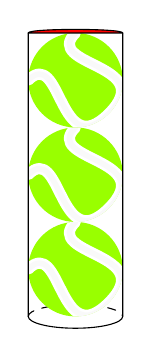
\begin{tikzpicture}[font=\footnotesize,line join=round, line cap=round, >=stealth,scale=0.6] 
			\tikzset{tenis/.pic={ 
					\clip [preaction={fill=green!40!yellow}] circle [radius=1];
					\draw [rotate=45, white, line width=4pt, postaction={draw=gray!5, line width=2pt}, line cap=round] 
					(270:1) .. controls ++(180:3/2) and ++(  0:1) ..(135:1)
					(270:1) .. controls ++(0  :3/2) and ++(180:1) ..( 45:1);
			}}
			\draw[dashed](-1,-1) arc(-180:-360:1cm and 0.25cm) (1,-1);	
			\path
			(0,0)pic[scale=0.6]{tenis}
			(0,2)pic[scale=0.6]{tenis}
			(0,4)pic[scale=0.6]{tenis}
			;
			\draw[fill=red] (-1,5) .. controls +(90:0.1) and +(90:0.1) .. (1,5)--cycle;
			\draw (-1,5)--(-1,-1) arc(180:360:1cm and 0.25cm) (1,-1)-- (1,5);
			
	\end{tikzpicture}}
	\loigiai{
		\begin{enumerate}
			\item Bán kính quả bóng là $R=\dfrac{6{,}5}{2}=3{,}25$\,(cm).\\
			Diện tích bề mặt mỗi quả bóng là $S=4\pi R^2=4\cdot \pi\cdot 3{,}25^2\approx 133$ $\left(\text{cm}^2\right)$.\\
			Thể tích của mỗi quả bóng là $V=\dfrac{4}{3}\pi R^3=\dfrac{4}{3}\cdot \pi\cdot 3{,}25^3 \approx 144$ $\left(\text{cm}^3\right)$.
			\item Hộp bóng là hình trụ có bán kính đáy cũng là bán kính quả bóng $R=3{,}25$\,cm và chiều cao $h=6R=19{,}5$\,cm.\\
			Diện tích xung quanh của hộp bóng là $S_{\text{xq}}=2\pi Rh=2\cdot \pi\cdot 3{,}25\cdot 19{,}5\approx 398$ $\left(\text{cm}^2\right)$.\\
			Thể tích của hộp bóng là $V=\pi R^2h=\pi\cdot 3{,}25^2\cdot 19{,}5\approx 647$ $\left(\text{cm}^3\right)$.\\
		\end{enumerate}
	} 
\end{bt}
\begin{bt}%[Dự án EX-9-Đề Cương Toán 9]%[Hoàng Thanh Phương]%[9H4H1-4]
	Một ly nước dạng hình trụ có chiều cao là $15$ cm, đường kính đáy là $5$ cm, lượng nước tinh khiết trong ly cao là $10$ cm.
	\immini{\begin{enumerate}
			\item Lượng nước được chứa trong ly là bao nhiêu cm$^3$? (Kết quả làm tròn đến hàng phần trăm)
			\item Người ta thả vào ly nước $5$ viên bi hình cầu có cùng thể tích, đồng chất và ngập hoàn toàn trong nước làm nước trong ly dâng lên bằng miệng ly. Hỏi bán kính của mỗi viên bi là bao nhiêu cm? (Kết quả làm tròn đến hàng phần trăm) (Giả sử độ dày của ly, đế ly là không đáng kể).
	\end{enumerate}}
	{\begin{tikzpicture}[line join=round,line cap=round,>=stealth,font=\footnotesize,scale=1,samples=300]
			\def\h{1.8}
			\def\a{1.3}
			\def\b{0.4}
			\fill[blue!30] (180:\a)--($(180:\a)+(90:\h)$)--($(0:\a)+(90:\h)$)--(0:\a)--cycle;
			\fill[blue!50] ($(180:\a)+(90:\h)$) arc (180:0:{\a} and {\b}) -- ($(0:\a)+(90:\h)$) arc (0:180:{\a} and {\b}) -- cycle;
			\filldraw[dashed,blue!50] (180:\a) arc(180:0:{\a} and {\b});
			\filldraw[blue!50] (180:\a) arc(180:360:{\a} and {\b});
			\filldraw[blue!50] ($(180:\a)+(90:\h)$) arc (180:0:{\a} and {\b});
			\filldraw[blue!50] ($(180:\a)+(90:\h)$) arc (180:360:{\a} and {\b});
			\filldraw[blue!50] (180:\a)--($(180:\a)+(90:\h)$) (0:\a)--($(0:\a)+(90:\h)$);
			\def\gA{0}
			\path
			(180:\a) arc (180:\gA:{\a} and {\b}) coordinate (A)
			($(A)+(90:\h)$)coordinate (A_1)
			($(A_1)+(0.5,0)$) coordinate (B1)
			($(A)+(0.5,0)$) coordinate (A1)
			($(A1)!0.5!(B1)$) node[right]{$10$ cm}
			;
			\draw[<->] (A1)--(B1);
			
			\def\h{3}
			\def\a{1.3}
			\def\b{0.4}
			\draw[dashed] (180:\a) arc(180:0:{\a} and {\b});
			\draw (180:\a) arc(180:360:{\a} and {\b});
			\draw ($(180:\a)+(90:\h)$) arc (180:0:{\a} and {\b});
			\draw ($(180:\a)+(90:\h)$) arc (180:360:{\a} and {\b});
			\draw (180:\a)--($(180:\a)+(90:\h)$) (0:\a)--($(0:\a)+(90:\h)$);
			\def\gA{0}
			\def\gB{180}
			\path
			(180:\a) arc (180:\gA:{\a} and {\b}) coordinate (A)
			(180:\a) arc (180:\gB:{\a} and {\b}) coordinate (B)
			\foreach \x in {A,B}{($(\x)+(90:\h)$) coordinate (\x_1)}
			($(B)+(0,-0.8)$) coordinate (B1)
			($(A)+(0,-0.8)$) coordinate (A1)
			($(A1)!0.5!(B1)$) node[below]{$5$ cm}
			($(B)+(-0.5,0)$) coordinate (C)
			($(B_1)+(-0.5,0)$) coordinate (C1)
			($(C)!0.5!(C1)$) node[left]{$15$ cm}
			;
			\draw[<->] (C)--(C1);
			\draw[<->] (A1)--(B1);
			\path (0,0) node{\hypersetup{hidelinks}\href{DaKIltf}{ }};
	\end{tikzpicture}}
	
	Biết rằng công thức tính thể tích hình trụ là $V=\pi\mathrm{r}^2h$ và công thức tính thể tích hình cầu là $V=\dfrac{4}{3}\pi\mathrm{R}^3$. Trong đó: $\mathrm{r}$ là bán kính đáy, $h$ là chiều cao hình trụ, $\mathrm{R}$ là bán kính của hình cầu và $\pi\approx3{,}14$.
	\loigiai{
		\begin{enumerate}
			\item Lượng nước chứa trong ly là
			$$V_1=\pi\mathrm{r}^2h=3{,}14\cdot\left(\dfrac{5}{2}\right)^2\cdot10\approx196{,}25 \,\left(\text{cm}^3\right).$$
			\item Lượng nước dâng lên bằng miệng ly chính là thể tích của cả $5$ viên bi nên thể tích của $5$ viên bi là
			$$V_2=\pi\mathrm{r}^2h=3{,}14\cdot\left(\dfrac{5}{2}\right)^2\cdot(15-10)\approx98{,}125\,\left(\text{cm}^3\right).$$
			Thể tích của một viên bi là
			$$\dfrac{V_2}{5}=\dfrac{98{,}125}{5}\approx 19{,}625\,\left(\text{cm}^3\right).$$
			Bán kính của một viên bi là
			$$\mathrm{R}=\sqrt[3]{\dfrac{3V}{4\pi}}=\sqrt[3]{\dfrac{3\cdot19{,}625}{4\cdot3{,}14}}\approx1{,}67 \text{ (cm)}.$$
		\end{enumerate}
	}
\end{bt}
\begin{bt}%[Dự án EX-9-Đề Cương Toán 9]%[Hoàng Thanh Phương]%[9H4B2-4]
	\immini{
		Một cái ly thủy tinh (như hình vẽ), phần phía trên là hình nón có chiều cao $7$ cm, có đáy đường tròn bán kính $4$ cm. Biết thể tích hình nón được tính theo công thức $V=\dfrac{1}{3} \pi r^2h$ với $r$ là bán kính đường tròn đáy của hình nón; $h$ là chiều cao của hình nón.
		\begin{enumerate}
			\item Tính thể tích của cái ly (bề dày của ly không đáng kể).
			\item Biết trong ly đang chứa rượu với mức rượu đang cách miệng ly là $3$ cm. Hỏi thể tích còn lại của ly rượu chiếm bao nhiêu phần của thể tích ly.
		\end{enumerate}
		\centering {(\textit{Lưu ý: kết quả làm tròn đến chữ số thập phân thứ hai, $\pi\approx 3{,}14$}).}
	}{
		\begin{tikzpicture}[scale=0.5]
			\coordinate (O) at (0,7);
			\coordinate (A) at (-4,7);
			\coordinate (B) at (-2.8,5);
			\coordinate (C) at (0,0);
			\coordinate (I) at (0,5);
			\coordinate (J) at (0,-4);
			\coordinate (D) at (0,7);
			
			\draw (O) -- (A) -- (C) -- (4,7);
			\draw (C) -- (J);
			\draw[fill=cyan!20] (B) arc (180:0:2.8 and 0.5) -- (C) -- cycle;
			
			\fill[left color=cyan!80, right color=cyan] (B) arc (180:0:2.8 and 0.5) -- (C) -- cycle;
			\draw (B) arc (180:360:2.8 and 0.5);
			\draw (J) ellipse (2 and 0.6);
			\draw (0,7) ellipse (4 and 0.6);
			\draw[dashed] (C) -- (I);
			\draw (O) -- (I) -- (B);
			
			\draw[|<->|] ($(A)+(0,1)$) -- ($(O)+(0,1)$) node[midway, above,scale=.8] {$4$ cm};
			\draw[|<->|] ($(A)+(-0.2,0)$) -- ($(-4,5)+(-0.2,0)$) node[midway, left,scale=.8] {$3$ cm};
			\draw[|<->|] ($(4,0)+(0.2,0)$) -- ($(4,7)+(0.2,0)$) node[midway, right,scale=.8] {$7$ cm};
			
			\foreach \x/\y/\z in {A/O/I, B/I/C} {
				\pic[draw, angle radius=6pt] {right angle = \x--\y--\z};
			} 
		\end{tikzpicture}	
	}
	\loigiai{
		Giả sử ta đặt tên điểm như hình vẽ bên
		\immini{
			\begin{enumerate}
				\item Theo đề $OA=4$ cm; $OC=7$ cm.\\ 
				Thể tích của cái ly là $$V=\dfrac{1}{3} \pi \cdot 4^2 \cdot 7=\dfrac{112\pi}{3}.$$ 
				\item Ta có $AO\parallel IB$ nên theo định lí Ta-lét thì 
				$$\dfrac{IB}{OA}=\dfrac{CI}{CO}\Rightarrow IB=\dfrac{OA\cdot CI}{CO}=\dfrac{4\cdot 4}{7}=\dfrac{16}{7} \,(\text{cm}^3).$$
				Thể tích rượu trong ly là
				$$V_1=\dfrac{1}{3} \pi \cdot IB^2 \cdot IC=\dfrac{1024\pi}{147}\,(\text{cm}^3).$$
				Thể tích phần còn lại trong ly (không chứa rượu) là
				$$V_2=V-V_1=\dfrac{112\pi}{3}-\dfrac{1024\pi}{147}=\dfrac{1844\pi}{49}\,(\text{cm}^3).$$
				Vậy thể tích còn lại của ly rượu chiếm $\dfrac{V_2}{V_1}\cdot 100\% \approx 81{,}34\%$ ly rượu.
			\end{enumerate}
		}{
			\begin{tikzpicture}[scale=0.5]
				\coordinate (O) at (0,7);
				\coordinate (A) at (-4,7);
				\coordinate (B) at (-2.8,5);
				\coordinate (C) at (0,0);
				\coordinate (I) at (0,5);
				\coordinate (J) at (0,-4);
				\coordinate (D) at (0,7);
				
				\draw (O) -- (A) -- (C) -- (4,7);
				\draw (C) -- (J);
				\draw[fill=cyan!20] (B) arc (180:0:2.8 and 0.5) -- (C) -- cycle;
				
				\fill[left color=cyan!80, right color=cyan] (B) arc (180:0:2.8 and 0.5) -- (C) -- cycle;
				\draw (B) arc (180:360:2.8 and 0.5);
				\draw (J) ellipse (2 and 0.6);
				\draw (0,7) ellipse (4 and 0.6);
				\draw[dashed] (C) -- (I);
				\draw (O) -- (I) -- (B);
				
				\draw[|<->|] ($(A)+(0,1)$) -- ($(O)+(0,1)$) node[midway, above,scale=.8] {$4$ cm};
				\draw[|<->|] ($(A)+(-0.2,0)$) -- ($(-4,5)+(-0.2,0)$) node[midway, left,scale=.8] {$3$ cm};
				\draw[|<->|] ($(4,0)+(0.2,0)$) -- ($(4,7)+(0.2,0)$) node[midway, right,scale=.8] {$7$ cm};
				
				\node[above left] at (A) {$A$};
				\node[left] at (B) {$B$};
				\node[below left] at (C) {$C$};
				\node[right] at (O) {$O$};
				\node[ right] at (I) {$I$};
				
				\foreach \x/\y/\z in {A/O/I, B/I/C} {
					\pic[draw, angle radius=6pt] {right angle = \x--\y--\z};
				} 
			\end{tikzpicture}	
		}
	}
\end{bt}
\begin{bt}%[Dự án EX-9-Đề Cương Toán 9]%[Hoàng Thanh Phương]%[9H4H1-4] 
	Một chiếc thùng đựng nước hình trụ có bán kính đáy là $15$ cm, đựng đầy nước. Khi vận chuyển lên xe thì thùng nước va vào một vật nhọn nên bị thủng một lỗ ở đáy thùng, khi di chuyển thì lỗ rò bắt đầu chảy nước với vận tốc chảy ra ngoài không đổi là $0{,}5$ lít/phút. Người đó chạy tới địa điểm giao nước mất $1$ giờ thì thấy rằng lúc tới nơi thì thùng vừa chảy hết nước. Tính chiều cao của thùng nước đó (làm tròn tới hàng phần mười, đơn vị đo là cm). Lấy $\pi\approx 3{,}14$.
	\loigiai{
		Thể tích thùng ban đầu là $0{,}5\cdot 60=30 ~(\text{lít})=30\,000 ~(\text{cm}^3)$. \\
		Ta có $V=\pi r^2h\Leftrightarrow 30\,000=\pi \cdot 15^2\cdot h \Leftrightarrow h\approx 30\,000=3{,}14\cdot 15^2 \cdot h\Leftrightarrow h\approx 42{,}5$ (cm).\\
		Vậy chiều cao của thùng nước ban đầu là $42{,}5$ cm.
	}
\end{bt}
\begin{bt}%[Dự án EX-9-Đề Cương Toán 9]%[Hoàng Thanh Phương]%[9H4H3-4]
	\immini
	{
		Một tháp nước có bể chứa hình cầu, đường kính bên trong của bể đo được là $6$ m.
		\begin{enumerate}
			\item Tính thể tích của tháp nước đó (theo đơn vị lít). 
			\item Biết rằng lượng nước đựng đầy trong bể đủ dùng cho khu dân cư trong $5$ ngày. Cho biết khu dân cư có $1\,304$ người. Hỏi trong một ngày mức bình quân mỗi người dùng là bao nhiêu lít nước? (lấy $\pi=3{,}14$, biết $1$ m$^3$ $=1000$ lít)
		\end{enumerate}
	}{\begin{tabular}{c c}
			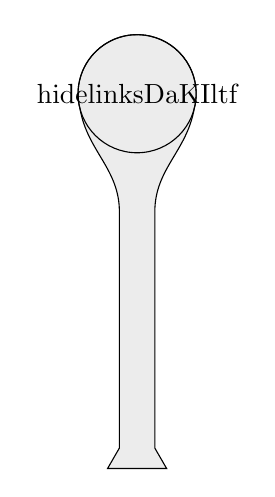
\begin{tikzpicture}[scale=0.75]
				\def\a{1}
				\path (0,0) coordinate (O)
				(-15:\a) coordinate (A)
				(195:\a) coordinate (B)
				(0.3,-2) coordinate (C);
				\fill[gray!15,draw=black](A)to[in=90,out=-100](C)--++(0,-4)--++(-60:0.4)--++(-1,0)--++(60:0.4)--++(0,4)to[in=-80,out=90](B)arc(195:-15:\a)--cycle;
				\draw (O) circle (\a);
				\path (0,0) node{\hypersetup{hidelinks}\href{DaKIltf}{ }};
			\end{tikzpicture}
			&
			\begin{tikzpicture}
				\def\a{2.5}
				\def\b{1.1}
				\path (0,0) coordinate (O)
				(\a,0) coordinate (A)
				(-\a,0) coordinate (B);
				\fill (O) circle (1pt);
				\draw (O) circle (\a) (B) arc (-180:0:{\a} and {\b});
				\draw[dashed] (A) arc (0:180:{\a} and {\b});
				\draw (O)--(A)node[above,midway]{$R$};
				\path (current bounding box.south)node[below]{$V=\dfrac{4}{3}\pi R^3$};
			\end{tikzpicture}
		\end{tabular}
	}
	\loigiai{
		\begin{enumerate}
			\item Bán kính của bể là $R=6:2=3$ (m).\\
			Thể tích của tháp nước là $V=\dfrac{4}{3}\pi R^3=\dfrac{4}{3}\cdot 3{,}14\cdot 3^3=113{,}04$ (m$^3$)$=113\,040$ (lít).\\
			\item Lượng nước bình quân mỗi người dùng trong năm ngày là $113\,040:1\,304=\dfrac{14\,130}{163}$ (lít).\\
			Lượng nước bình quân mỗi người dùng trong một ngày là $\dfrac{14\,130}{163}:5 = \dfrac{2826}{163} \approx 17$ (lít).\\
			Vậy bình quân mỗi người dùng khoảng $17$ lít nước trong một ngày.
		\end{enumerate}
	}
\end{bt}
\begin{bt}%[Dự án EX-9-Đề Cương Toán 9]%[Hoàng Thanh Phương]%[9H4B1-4]
	Một khối gỗ hình trụ có bán kính đáy là $3$ cm, chiều cao $4$ cm được đặt đứng trên mặt bàn. Một phần của khối gỗ bị cắt rời theo các bán kính $OA$, $OB$ và theo chiều dài thẳng đứng từ trên xuống dưới với $\widehat{AOB}=30^\circ$ như hình vẽ bên dưới
	\begin{center}
		\begin{tikzpicture}[scale=1,>=stealth, font=\footnotesize, line join=round, line cap=round]
			\def \x{1.8}%bán kính trục lớn elip
			\def \y{0.8}%bán kính trục bé elip
			\def \h{-2.5}%chiều cao hình trụ
			\path (0,0) coordinate (O)
			($(O)+(0,\h)$) coordinate (O')
			($(O)+(\x,0)$) coordinate (P)
			($(O)+(-\x,0)$) coordinate (Q)
			($(O')+(\x,0)$) coordinate (P')
			($(O')+(-\x,0)$) coordinate (Q')
			($(O)+({\x*cos(-65)},{\y*sin(-70)})$) coordinate (A)
			($(O)+({\x*cos(-115)},{\y*sin(-110)})$) coordinate (B)
			($(B)+(0,\h)$) coordinate (B')
			($(A)+(0,\h)$) coordinate (A')
			;
			\fill[fill=brown!40!] (A)--(O)--(O')--(A')
			(B)--(O)--(O')--(B')
			;
			\draw[fill=brown!20!] (B') arc(-115:-65:\x cm and \y cm)--(A)arc(-65:-115:\x cm and \y cm)--(B)--cycle;
			\draw (B) arc(-115:-65:\x cm and \y cm);
			\draw(A')--(A)--(O)--(B)--(B')
			(A)--(O)--(B)
			;
			\draw[dashed](O)--(O')--(A')(O')--(B');			
			\foreach \p/\r in {O/90,A/-45,B/-135}
			\fill (\p) circle (1pt) node[shift={(\r:3mm)}]{$\p$};
			\draw pic[fill=yellow,draw=black,opacity=.5, angle eccentricity=1.2, angle radius=0.3cm]{angle=B'--O'--A'};
			\path (O') node[shift={(-90:5mm)}]{$30^\circ$};
			\path (O)--(O')node[pos=.6,sloped,below =-2pt]{$4$ cm}
			(O)--(A)node[midway,right]{$3$ cm}
			;
		\end{tikzpicture}\hspace*{1cm}		
		\begin{tikzpicture}[scale=1,>=stealth, font=\footnotesize, line join=round, line cap=round]
			\def \x{1.8}%bán kính trục lớn elip
			\def \y{0.8}%bán kính trục bé elip
			\def \h{-2.5}%chiều cao hình trụ
			\path (0,0) coordinate (O)
			($(O)+(0,\h)$) coordinate (O')
			($(O)+(\x,0)$) coordinate (P)
			($(O)+(-\x,0)$) coordinate (Q)
			($(O')+(\x,0)$) coordinate (P')
			($(O')+(-\x,0)$) coordinate (Q')
			($(O)+({\x*cos(-65)},{\y*sin(-70)})$) coordinate (A)
			($(O)+({\x*cos(-115)},{\y*sin(-110)})$) coordinate (B)
			($(B)+(0,\h)$) coordinate (B')
			($(A)+(0,\h)$) coordinate (A')
			;
			\fill[fill=brown!20!] (P') arc(0:360:\x cm and \y cm);
			\fill[fill=brown!20!] (P)--(P')--(Q')--(Q)--cycle;
			\draw[fill=brown!40!] (A) arc(-65:245:\x cm and \y cm);
			\fill[fill=brown!40!] (A)--(O)--(O')--(A')
			(B)--(O)--(O')--(B')
			;
			\fill[fill=white] (B')arc(-115:-65:\x cm and \y cm)--(A')--(O')--cycle;
			\draw[dashed] (P') arc(0:180:\x cm and \y cm);
			\draw(A') arc(-65:0:\x cm and \y cm);
			\draw(Q') arc(180:245:\x cm and \y cm);
			\draw(P)--(P')(Q)--(Q')
			(A)--(O)--(B)--(B')--(O')--(A')--(A)
			;
			\draw[dashed](O)--(O');			
			\foreach \p/\r in {O/90,A/-45,B/-135}
			\fill (\p) circle (1pt) node[shift={(\r:3mm)}]{$\p$};
			\draw pic[fill=yellow,draw=black,opacity=.5, angle eccentricity=1.2, angle radius=0.3cm]{angle=B'--O'--A'};
			\path (O') node[shift={(-90:5mm)}]{$30^\circ$};
			\path (O)--(O')node[midway,sloped,below=-2pt]{$4$ cm}
			(O)--(A)node[midway,right]{$3$ cm}
			;
		\end{tikzpicture}
	\end{center}
	\begin{enumerate}
		\item Tính thể tích của khối gỗ còn lại sau khi bị cắt rời. \textit{(kết quả làm tròn đến phần mười)}
		\item Diện tích toàn phần của khối gỗ còn lại sau khi đã bị cắt.	\textit{(kết quả làm tròn đến phần mười)}
	\end{enumerate}
	\loigiai{
		\begin{enumerate}
			\item Thể tích khối gỗ còn lại sau khi bị cắt rời là
			$$
			\dfrac{360-30}{360}\cdot V_{\text{khối gỗ}}
			=\dfrac{11}{12}\cdot \pi \cdot 3^2\cdot 4
			=33\pi \approx 103{,}7 \text{ (cm$^3$)}.
			$$
			Vậy thể tích khối gỗ còn lại khoảng $103{,}7$ cm$^3$.
			\item  Diện tích toàn phần của khối gỗ còn lại sau khi đã bị cắt là
			\begin{eqnarray*}
				\dfrac{360-30}{360}\cdot \left(S_{\text{toàn phần}}+2S_\text{đáy}\right)+2S_{\text{hcn}}
				&=&\dfrac{11}{12}\cdot \left(2\cdot \pi \cdot 3\cdot 4+2\cdot \pi \cdot 3^2\right)+2\cdot 3\cdot 4\\
				&=&\dfrac{77}{2}\pi+24\approx 93{,}1\text{ (cm$^2$)}
			\end{eqnarray*}
			Vậy diện tích toàn phần của khối gỗ là $93{,}1$ (cm$^2$).
		\end{enumerate}
	}
\end{bt}
\begin{bt}%[Dự án EX-9-Đề Cương Toán 9]%[Hoàng Thanh Phương]%[9H4H1-4]
	\immini{
		Một thùng đựng nước có dạng hình trụ với chiều cao là $35$ cm và đường kính đáy là $30$ cm.
		\begin{enumerate}
			\item Tính thể tích của thùng nước. (\textit{kết quả làm tròn đến hàng đơn vị}).
			\item Người ta sử dụng thùng nước trên để múc nước đổ vào một bể chứa có dung tích $1$ m$^3$. Hỏi cần phải đổ ít nhất bao nhiêu thùng nước thì đầy bể chứa? Biết rằng, mỗi lần xách người ta chỉ đổ đầy $90\%$ thùng để nước không đổ ra ngoài. Cho công thức tính thể tích hình trụ: $V=\pi r^2 \cdot h$ trong đó $h$ là chiều cao hình trụ, $r$ là bán kính đường tròn đáy.
		\end{enumerate}
	}{
		\begin{tikzpicture}[>=stealth,line join=round,line cap=round,font=\footnotesize,scale=1]
			\def\x{1.4}
			\def\y{0.6}
			\coordinate (O) at (0,0);
			\coordinate (O') at ($(O)+(0,3.1)$);
			\coordinate (N) at ($(O)+(0,3)$);
			\path[fill=cyan!40] (N) arc (0:180:\x cm and \y cm)--($(O)+(-2*\x,0)$) arc (180:360:\x cm and \y cm) --cycle;
			\draw[dashed,blue] (N) arc (0:180:\x cm and \y cm);
			%\node[circle,outer color=white!80!black,inner color=white,minimum width=1.2cm] (radial) at (-5.7,2.5) {};
			\draw[dashed,blue] (N) arc (0:-180:\x cm and \y cm);
			%\draw[dashed] (O) arc (0:180:\x cm and \y cm);
			\draw (O) arc (0:-180:\x cm and \y cm);
			
			\draw (O)--(O') ($(O)+(-2*\x,0)$)--($(O')+(-2*\x,0)$);
			
			\fill (N) circle(2pt) node{$N$};
			\path[fill=cyan!40] (0.3,3.1) arc (0:180:1.7 cm and 0.6 cm)--(-3.1,2.6) arc (180:360:1.7 cm and 0.6 cm) --cycle;
			\draw (0.3,3.1) arc (0:180:1.7 cm and 0.6 cm)--(-3.1,2.6) arc (180:360:1.7 cm and 0.6 cm) --cycle;
			\draw (-3.1,3.1) arc (180:360:1.7 cm and 0.6 cm);
			\draw (O') arc (0:360:\x cm and 0.45 cm);
			\fill[cyan!10] (O') arc (0:360:\x cm and 0.45 cm);
		\end{tikzpicture}
	}
	\loigiai{
		\begin{enumerate}
			\item Thể tích của thùng nước là
			$$V=\pi \cdot\left(\dfrac{30}{2}\right)^2 \cdot 35=7\,875 \pi \approx 24\,740\, \left(\mathrm{cm}^3\right).
			$$
			\item Đổi $1$ m$^3=1\,000\,000$ cm$^3$.\\
			Số thùng nước ít nhất cần phải đổ để đầy bể chứa là
			$$1\,000\,000:(7\,875 \pi \cdot90 \%) \approx 45 \textrm{ (thùng).}$$
			Vậy cần phải đổ ít nhất $45$ thùng nước thì đầy bể chứa.
		\end{enumerate}
	}
\end{bt} 
\begin{bt}%[Dự án EX-9-Đề Cương Toán 9]%[Hoàng Thanh Phương]%[9H4H2-4]
	Cái mũ có vành của chú hề với các kích thước cho theo hình vẽ
	\begin{center}
		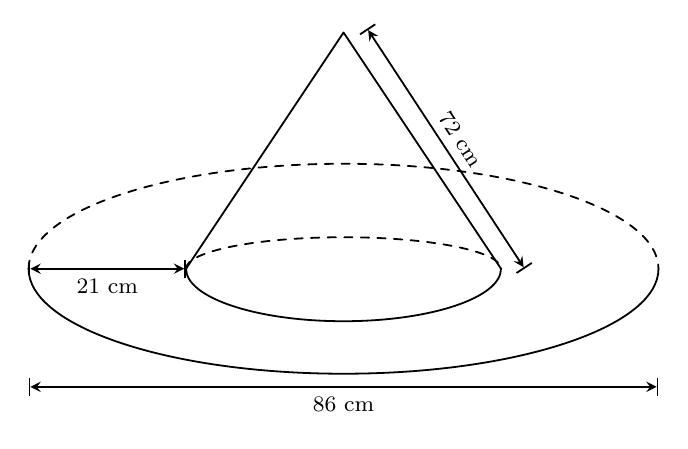
\begin{tikzpicture}[scale=1,>=stealth, font=\footnotesize, line join=round, line cap=round,line width=0.65pt]
			\def\a{2}
			\def\b{4}
			\def\h{3}
			\path (0:0) coordinate (O)
			(180:{\a} and {\a/3}) coordinate (A)
			(0:{\a} and {\a/3}) coordinate (B)
			(O)+(0,\h) coordinate (S)
			(0,0)+(180:{\b} and {\b/3}) coordinate (C)
			(-2,0)+(0:{\b} and {\b/3}) coordinate (D)
			;
			\draw (A) arc (180:360:{\a} and {\a/3}) (A)--(S)--(B) (C) arc (180:360:{\b} and {\b/3});
			\draw[dashed] (A) arc (-180:-360:{\a} and {\a/5}) (C) arc (-180:-360:{\b} and {\b/3});
			\draw[|<->|] (-2,0)--(-4,0) node[below,pos=0.5,sloped]{$21$ cm};
			\draw[|<->|] (-4,-1.5)--(4,-1.5) node[below,pos=0.5,sloped]{$86$ cm};
			\draw[|<->|] (2.3,0)--(0.3,3.05) node[above,pos=0.5,sloped]{$72$ cm};
		\end{tikzpicture}
	\end{center}
	\begin{enumerate}
		\item Hãy tính tổng diện tích vải cần có để làm nên cái mũ của chú hề (không kể riềm, mép, phần thừa).
		\item Chú hề dự định mua bột đổ đầy nón để làm ảo thuật. Chú hề cần mua khối lượng bột là bao nhiêu (làm tròn đến hàng đơn vị)? (biết rằng khối lượng riêng của loại bột đó là $1$ g/cm$^3$ nghĩa là $1$ cm$^3$ tương ứng với $1$ g).
		Cho công thức tính thể tích hình nón $V=\dfrac{1}{3}\pi r^2h$.\\  
		Công thức tính dện tích xung quanh hình nón là $S_{\textrm{xq}}=\pi rl$.\\
		Trong đó $h$ là chiều cao hình nón, $r$ là bán kính đáy, $l$ là đường sinh, $\pi\approx3{,}14$.
	\end{enumerate}
	\loigiai
	{
		\begin{enumerate}
			\item Bán kính hình nón là $r=\dfrac{86-21\cdot2}{2}=22$ (cm).\\
			Diện tích xung quanh là $S_{\textrm{xq}}=\pi rl=3{,}14\cdot22\cdot72=4\,973{,}76$ (cm$^2$).\\
			Diện tích vành nón là $S_{\textrm{vn}}=\pi\cdot\left(\dfrac{86}{2}\right)^2-\pi\cdot22^2=4\,286{,}1$ (cm$^2$).\\
			Diện tích cần tìm là $S=S_{\textrm{xq}}+S_{\textrm{vn}}=4\,973{,}76+4\,286{,}1=9\,259{,}86$ (cm$^2$).\\
			Vậy tổng diện tích vải cần có để làm nên cái mũ của chú hề (không kể riềm, mép, phần thừa) gần bằng $9\,259{,}86$ cm$^2$.
			\item Chiều cao hình nón $h=\sqrt{72^2-22^2}=10\sqrt{47}$ (cm).\\
			Thể tích hình nón $V=\dfrac{1}{3}\pi r^2h=\dfrac{1}{3}\cdot3{,}14\cdot22^2\cdot10\sqrt{47}\approx34\,729{,}8$ (cm$^3$).\\
			Vậy số bột cần để đổ đầy nón là $34\,730$ (g).
		\end{enumerate}
	}
\end{bt} 
\begin{bt}%[Dự án EX-9-Đề Cương Toán 9]%[Hoàng Thanh Phương]%[9H4V2-4]
	\immini {
		Một chai nước suối của hãng A được thiết kế gồm $3$ phần: phần miệng chai có dạng hình trụ với chiều cao $2{,}5$ cm và đường kính đường tròn đáy là $3$ cm, phần cổ chai có dạng hình nón cụt với chiều cao $5$ cm, phần thân chai có dạng hình trụ với chiều cao $10$ cm và đường kính đường tròn đáy là $6$ cm.
		\begin{enumerate}
			\item Tính thể tích chai nước (làm tròn đến hàng đơn vị) biết công thức tính thể tích hình trụ là $V=\pi R^2h$, thể tích hình nón cụt là $V=\dfrac{1}{3} \pi h \cdot\left(r_1^2+r_2^2+r_1r_2\right)$.
			\item Người ta đóng nước vào chai, và để tránh tình trạng giãn nở vì nhiệt nhà sản xuất chỉ đóng vào chai một lượng nước bằng $90\%$ thể tích chai nước. Đồng thời Viện y tế quốc gia Hoa Kỳ (NIH) khuyến nghị mỗi người nên uống đủ $2$ lít nước mỗi ngày. Hỏi cần mua tối thiểu bao nhiêu chai nước suối của hãng A để đảm bảo theo khuyến nghị của NIH?
		\end{enumerate}
	}{
		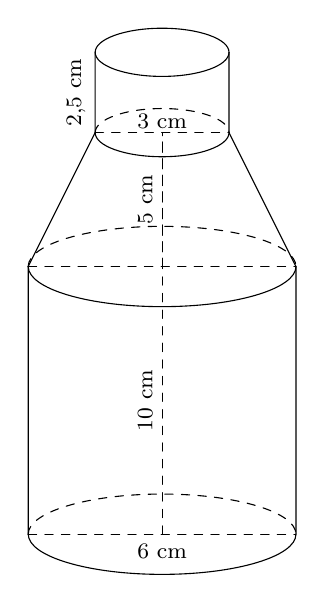
\begin{tikzpicture}[scale=0.85, font=\footnotesize,line join=round, line cap=round, >=stealth]	
			\def\ra{2} \def\rb{1} \def\cao{4} \def\rong{0.6};
			\draw[dashed] (-\ra,0) arc (180:0:{\ra} and {\rong});
			\draw[] (-\ra,0) arc (180:360:{\ra} and {\rong});
			\draw[dashed] (-\ra,\cao) arc (180:0:{\ra} and {\rong});
			\draw[] (-\ra,\cao) arc (180:360:{\ra} and {\rong});
			\draw[dashed] (-\rb,1.5*\cao) arc (180:0:{\rb} and {0.6*\rong});
			\draw[] (-\rb,1.5*\cao) arc (180:360:{\rb} and {0.6*\rong});
			\draw (0,1.8*\cao) ellipse ({\rb} and {0.6*\rong});
			\draw [dashed](0,0)--(0,\cao) node[pos=0.5,sloped,above]{$10$ cm}
			(0,\cao)--(0,1.5*\cao) node[midway,sloped,above]{$5$ cm}
			(-\rb,1.5*\cao)--(\rb,1.5*\cao)node[pos=0.5,sloped,yshift=4]{$3$ cm}
			(-\ra,0)--(\ra,0)node[pos=0.5,sloped,below]{$6$ cm}
			(-\ra,\cao)--(\ra,\cao)
			(0,0)--(0,1.5*\cao)
			;
			\draw [](-\rb,1.5*\cao)--(-\rb,1.8*\cao)node[pos=0.5,sloped,above]{$2{,}5$ cm}
			(-\ra,0)--(-\ra,\cao)--(-\rb,1.5*\cao)
			(\ra,0)--(\ra,\cao)--(\rb,1.5*\cao)--(\rb,1.8*\cao)
			;		
		\end{tikzpicture}
	}	
	\loigiai{		
		\begin{enumerate}
			\item Thể tích chai nước			
			$$\pi \cdot 1{,}5^2\cdot 2{,}5+\dfrac{1}{3} \pi \cdot 5\cdot\left(1{,}5^2+3^2+1{,}5\cdot 3\right)+\pi \cdot 3^2\cdot 10\approx 383\text{ (cm$^3$)}.$$
			\item $2$ lít $=2\,000$ (cm$^3$).\\		
			Lượng nước trong $1$ chai 		
			$$383\cdot 90\%=344{,}7\text{ (cm$^3$)}.$$
			Vì $2\,000: 344{,}7\approx 5{,}8$, nên ta cần mua tối thiểu $6$ chai nước.
		\end{enumerate}		
	}
\end{bt} 
\begin{bt}%[Dự án EX-9-Đề Cương Toán 9]%[Hoàng Thanh Phương]%[9H4H4-2]
	Một bồn nước hình trụ có đường kính đáy là $1{,}4$ (m) và cao $3{,}25$ (m). Người ta đổ nước vào trong bồn sao cho chiều cao của nước bằng đúng một nửa chiều cao của bồn và tiếp tục đặt vào trong bồn một phao nước có dạng hình cầu bằng kim loại không thấm nước có bán kính $30$ (cm) và chìm hoàn toàn vào trong nước.
	\begin{enumerate}
		\item Tính thể tích nước có trong bồn (\textit{kết quả làm tròn đến hàng phần mười}).
		\item Sau đó người ra tiếp tục bơm thêm nước vào bồn bằng một vòi có công suất chảy là $0{,}0024$ (m$^3$) cho mỗi giây. Hỏi sau bao nhiêu phút thì bồn đầy nước?\\
		Biết công thức tính thể tích hình trụ là $V=\pi r^2h$, công thức tính thể tích hình cầu là $V=\dfrac{4}{3}\pi R^3$, kết quả làm tròn đến hàng đơn vị.
	\end{enumerate}
	\loigiai{
		\begin{enumerate}
			\item Bán kính đáy của bồn là $r = 1{,}4:2=0{,}7$ (m).\\
			Thể tích nước có trong bồn là 
			$$V_1 = \dfrac{1}{2}\pi r^2h = \dfrac{1}{2} \pi\cdot0{,}7^2\cdot 3{,}25 = \dfrac{637\pi}{800} \approx 2{,}5 \text{ (m$^3$).}$$ 
			\item Đổi đơn vị: $30$ cm $= 0{,}3$ m.\\
			Tổng thể tích nước có trong bồn và thể tích của phao nước hình cầu là $$V_2 = V_1 + V_{\text{phao nước}} = \dfrac{637\pi}{800} +  \dfrac{4}{3} \pi\cdot 0{,}3^3 = \dfrac{3\,329\pi}{4\,000} \text{ (m$^3$).}$$
			Thể tích nước cần bơm để bồn đầy nước là 
			$$ \pi\cdot0{,}7^2\cdot 3{,}25 - \dfrac{3\,329\pi}{4\,000} = \dfrac{3\,041\pi}{4\,000} \text{ (m$^3$).}$$
			Thời gian để bồn đầy nước là $\dfrac{3\,041\pi}{4\,000}:0{,}0024 = \dfrac{15\,205\pi}{48}$ (giây) $\approx 17$ (phút).\\
			Vậy sau khoảng $17$ phút thì bồn sẽ đầy nước.
		\end{enumerate}
	}
\end{bt}
\begin{bt}%[Dự án EX-9-Đề Cương Toán 9]%[Hoàng Thanh Phương]%[9H4H4-3]
	\immini{
		Cho hình bên là một thúng gạo vun đầy. Thúng có dạng nửa hình cầu với đường kính $50$ cm, phần gạo vun lên có dạng hình nón cao $15$ cm.
		\begin{enumerate}
			\item Tính thể tích phần gạo trong thúng (\textit{làm tròn đến phần mười}).\\
			Biết thể tích hình nón là $V=\dfrac{1}{3}\pi R^2h$, hình trụ là $V=\pi R^2h$ và hình cầu là $V=\dfrac{4}{3}\pi R^3$.
			\item Nhà Dũng dùng lon sữa bò cũ có dạng hình trụ (bán kính đáy bằng $5$ cm, chiều cao $15$ cm) để đong gạo mỗi ngày. Biết mỗi ngày nhà Dũng ăn $5$ lon gạo và mỗi lần đong thì lượng gạo chiếm $90\%$ thể tích lon. Hỏi với lượng gạo ở thúng trên thì nhà Dũng có thể ăn nhiều nhất là bao nhiêu ngày?
		\end{enumerate} 
	}{
		\begin{tikzpicture}[line join = round, line cap=round,>=stealth,font=\footnotesize,scale=1]
			\tikzset{gao/.pic={
					\filldraw[white!70] (0,0) ellipse (2cm and 1cm);
					\draw[] (0,0) ellipse (2cm and 1cm);
			}}
			%\foreach \p/\r in {A/0,B/0,C/0}
			%\fill (\p) circle (1.2pt) node[shift={(\r:3mm)}]{$\p$};
			\begin{scope}[xshift=-4.3cm]
				\fill[brown!90] (0,0) arc (0:-180:2 and 2)-- (-4,0) arc(0:-180:-2 and 0.4) --cycle ;
				\draw [dashed](0,0) arc(0:180:2 and 0.4) ;
				\draw (0,0) arc(0:-180:2 and 0.4) ;
				\draw (0,0) arc(0:-180:2 and 2);
				\draw (-3.9,0)--(-2,2)--(-0.1,0);
				%	\begin{scope}[white!95!black!200]
					%	\clip (-3.9,0)--(-2,2)--(-0.1,0);	
					%	\foreach \i in {0.1,0.2,...,3.9} {
						%	\pgfmathsetmacro\r{0.05}
						%	\path 
						%	(-\i,\r*0) pic[scale=0.02]{gao}
						%	(-\i,\r*1) pic[scale=0.02]{gao}
						%	(-\i,\r*2) pic[scale=0.02]{gao}
						%	(-\i,\r*3) pic[scale=0.02]{gao}
						%	(-\i,\r*4) pic[scale=0.02]{gao}
						%	(-\i,\r*5) pic[scale=0.02]{gao}
						%	(-\i,\r*6) pic[scale=0.02]{gao}
						%	(-\i,\r*7) pic[scale=0.02]{gao}
						%	(-\i,\r*8) pic[scale=0.02]{gao}
						%	(-\i,\r*9) pic[scale=0.02]{gao}
						%	(-\i,\r*10) pic[scale=0.02]{gao}
						%	(-\i,\r*11) pic[scale=0.02]{gao}
						%	(-\i,\r*12) pic[scale=0.02]{gao}
						%	(-\i,\r*13) pic[scale=0.02]{gao}
						%	(-\i,\r*14) pic[scale=0.02]{gao}
						%	(-\i,\r*15) pic[scale=0.02]{gao}
						%	(-\i,\r*16) pic[scale=0.02]{gao}
						%	(-\i,\r*17) pic[scale=0.02]{gao}
						%	(-\i,\r*18) pic[scale=0.02]{gao}
						%	(-\i,\r*19) pic[scale=0.02]{gao}
						%	(-\i,\r*20) pic[scale=0.02]{gao}
						%	(-\i,\r*21) pic[scale=0.02]{gao}
						%	(-\i,\r*22) pic[scale=0.02]{gao}
						%	(-\i,\r*23) pic[scale=0.02]{gao}
						%	(-\i,\r*24) pic[scale=0.02]{gao}
						%	(-\i,\r*25) pic[scale=0.02]{gao}
						%	(-\i,\r*26) pic[scale=0.02]{gao}
						%	(-\i,\r*27) pic[scale=0.02]{gao}
						%	(-\i,\r*28) pic[scale=0.02]{gao}
						%	(-\i,\r*29) pic[scale=0.02]{gao}
						%	(-\i,\r*30) pic[scale=0.02]{gao}
						%	(-\i,\r*31) pic[scale=0.02]{gao}
						%	(-\i,\r*32) pic[scale=0.02]{gao}
						%	(-\i,\r*33) pic[scale=0.02]{gao}
						%	(-\i,\r*34) pic[scale=0.02]{gao}
						%	(-\i,\r*35) pic[scale=0.02]{gao}
						%	(-\i,\r*36) pic[scale=0.02]{gao}
						%	(-\i,\r*37) pic[scale=0.02]{gao}
						%	(-\i,\r*38) pic[scale=0.02]{gao}
						%	(-\i,\r*39) pic[scale=0.02]{gao}
						%	(-\i,\r*40) pic[scale=0.02]{gao}
						%	;
						%	}
					%	\end{scope}	
				%	\begin{scope}[white!95!black!200]
					%	\clip	(-3.9,0) arc (0:-180:-1.9cm and 0.45cm)--(-0.1,0)--cycle;
					%	\foreach \i in {0.1,0.2,...,3.9} {
						%	\pgfmathsetmacro\r{-0.05}
						%	\path 
						%	(-\i,\r*0) pic[scale=0.02]{gao}
						%	(-\i,\r*1) pic[scale=0.02]{gao}
						%	(-\i,\r*2) pic[scale=0.02]{gao}
						%	(-\i,\r*3) pic[scale=0.02]{gao}
						%	(-\i,\r*4) pic[scale=0.02]{gao}
						%	(-\i,\r*5) pic[scale=0.02]{gao}
						%	(-\i,\r*6) pic[scale=0.02]{gao}
						%	(-\i,\r*7) pic[scale=0.02]{gao}
						%	(-\i,\r*8) pic[scale=0.02]{gao}
						%	(-\i,\r*9) pic[scale=0.02]{gao}
						%	;
						%	}
					%	\end{scope}
			\end{scope}
			\draw [dashed](0,0) arc(0:180:2 and 1) ;
			\draw (0,0) arc(0:-180:2 and 1) ;
			\draw (0,0) arc(0:-180:2 and 2);
			\draw (-4,0)--(-2,3)--(0,0);
			\draw[dashed] (-2,3)coordinate (H)--(-2,0)coordinate (O) (-4,0)coordinate (A)--(0,0)coordinate (B);
			\draw pic[draw,angle radius=3mm] {right angle = H--O--B}; 
			\draw (0,0) arc(0:40:2 and 1);
			\draw (-4,0) arc(0:40:-2 and 1);
			\path[] (A)--(B) node[pos=0.5,below]{$50$ cm};
			\path[] (H)--(O) node[pos=0.5,right]{$12$ cm};
		\end{tikzpicture}
	}
	\loigiai
	{
		\begin{enumerate}
			\item Bán kính của thúng gạo là $50:2=25$ (cm).\\
			Thể tích phần gạo trong thúng là
			$$V=\dfrac{1}{2}\cdot\dfrac{4}{3}\pi R^3+\dfrac{1}{3}\pi R^2h=\dfrac{1}{2}\cdot\dfrac{4}{3}\pi \cdot25^3+\dfrac{1}{3}\pi\cdot25^2\cdot15 = \dfrac{40625}{3}\pi \approx 42542{,}4\, (\text{cm}^3).$$
			\item Thể tích gạo nhà bạn Dũng ăn một ngày là 
			$$V'=90\% \pi R^2h\cdot5=90\%\pi\cdot 5^2\cdot15\cdot5 = \dfrac{3375}{2}\pi\, (\text{cm}^3).$$
			Số ngày nhà bạn Dũng ăn hết thúng gạo là
			$$ \left(\dfrac{40625}{3}\pi\right) : \left(\dfrac{3375}{2}\pi\right) \approx 8\, (\text{ngày}).$$
			Vậy với lượng gạo ở thúng trên thì nhà Dũng có thể ăn nhiều nhất là $8$ ngày. 
		\end{enumerate} 
	}
\end{bt} 
\begin{bt}%[Dự án EX-9-Đề Cương Toán 9]%[Hoàng Thanh Phương]%[9H4H1-4]
	Nước giải khát thường đựng trong lon nhôm và cỡ lon phổ biến trên thế giới thường chứa được khoảng $330$ (ml) chất lỏng, được thiết kế hình trụ với chiều cao $10{,}2$ (cm), đường kính đường tròn đáy $6{,}42$ (cm). Nhưng hiện nay các nhà sản xuất có xu hướng tạo ra những lon nhôm với kiểu dáng thon cao. Tuy chi phí sản xuất của những chiếc lon này tốn kém hơn, do nó có diện tích mặt ngoài lớn hơn, nhưng nó lại dễ đánh lừa thị giác và được người tiêu dùng ưa chuộng hơn.
	\begin{enumerate}
		\item Một lon nước ngọt hiện nay có dạng hình trụ cao $13{,}41$ (cm), đường kính đường tròn đáy là $5{,}6$ (cm). Hỏi lon nước ngọt hiện nay có thể chứa được hết lượng nước ngọt của một lon có cỡ phổ biến không? Vì sao?
		\item Hỏi chi phí sản xuất lon nước ngọt hiện nay ở câu a) tăng bao nhiêu phần trăm so với chi phí sản xuất lon có cỡ phổ biến (biết chi phí sản xuất tỉ lệ thuận với diện tích toàn phần của lon)?
	\end{enumerate}
	\loigiai
	{
		\begin{enumerate}
			\item Thể tích của lon nước ngọt hiện nay là
			$$ \pi \cdot r_2^2 \cdot h_2 = 3{,}14 \cdot \left( \dfrac{5{,}6}{2} \right)^2 \cdot 13{,}41 = 330{,}122016 \text{ (cm$^3$).} = 330{,}122016 \text{ (ml).} $$
			Vì $330{,}122016 > 330$ nên lon nước ngọt hiện nay có thể chứa hết lượng nước của lon cỡ phổ biến.
			\item Diện tích toàn phần của lon nước ngọt có cỡ phổ biến là
			$$ S_1 = S_{\textrm{xq}_1} + 2S_{\textrm{đáy}_1} \approx 3{,}14 \cdot 6{,}42 \cdot 10{,}2 + 2\cdot 3{,}14\cdot \left( \dfrac{6{,}42}{2} \right)^2 \approx 270{,}3 \text{ (cm$^2$).} $$
			Diện tích toàn phần của lon nước ngọt hiện nay là
			$$ S_2 = S_{\textrm{xq}_2} + 2S_{\textrm{đáy}_2} \approx 3{,}14 \cdot 5{,}6 \cdot 13{,}41 + 2\cdot 3{,}14 \cdot \left( \dfrac{5{,}6}{2} \right)^2 \approx 285{,}0 \text{ (cm$^2$).} $$
			Phần trăm chi phí sản xuất thay đổi là
			$$ \dfrac{S_2 - S_1}{S_1} \cdot 100\% = \dfrac{285{,}0 - 270{,}3}{270{,}3} \cdot 100\% \approx 5{,}4\%. $$
			Vậy chi phí sản xuất lon nước ngọt hiện nay thực tế tăng khoảng $5{,}4\%$ so với chi phí sản xuất lon có cỡ phổ biến.
		\end{enumerate}
	}
\end{bt} 
\begin{bt}%[Dự án EX-9-Đề Cương Toán 9]%[Hoàng Thanh Phương]%[9H4H4-2]
	\immini{Một hãng sản xuất rượu vang đã đặt hàng một công ty sản xuất thủy tinh một kiểu ly có phần đựng rượu cao $6$ m, đường kính miệng ly là $6$ cm. Biết rằng để tạo thành ly là sự kết hợp gồm thành ly là một hình trụ cao $3$ cm, phần đáy ly là một nửa khối cầu có đường kính bằng với đường kính của miệng ly.  
		\begin{enumerate}
			\item Hãy tính thể tích rượu được chứa tối đa khi đổ vào ly? \\  
			Cho biết 
			\begin{itemize}
				\item $V_{\text{trụ}} = \pi r^2 h$ với $r$ là bán kính đáy, $h$ là chiều cao hình trụ.
				\item $V_{\text{cầu}} = \dfrac{4}{3} \pi R^3$ với $R$ là bán kính hình cầu. 
			\end{itemize} 
			\item Ông A cần chuẩn bị một số chai rượu vang, lượng rượu trong mỗi chai là $0{,}85$ lít. Biết rằng trong bữa tiệc có $12$ người (bao gồm luôn ông A), mỗi người uống $4$ ly rượu, lượng rượu được rót bằng $60\%$ thể tích của ly. Ông A cần chuẩn bị ít nhất bao nhiêu chai rượu vang?
		\end{enumerate}
		
	}{\begin{tikzpicture}[line join = round, line cap=round,>=stealth,font=\footnotesize,scale=0.7]
			\path 
			(0,0) coordinate (O)
			($(O)+(0.5,0)$) coordinate (O1)
			($(O)+(-4.5,0)$) coordinate (O2)
			% ($(O)+(2,0)$) coordinate (O1)
			(-2,-3.75) coordinate (O')
			($(O')+(0.6,0)$) coordinate (O1')
			($(O')+(-0.6,0)$) coordinate (O2')
			(-2,-8.5) coordinate (O'')
			($(O'')+(0.6,0)$) coordinate (O1'')
			($(O'')+(-0.6,0)$) coordinate (O2'')
			;
			\draw
			(O) arc(0:180:2cm and 0.5 cm)
			(O) arc(0:-180:2cm and 0.5 cm)
			;
			\draw
			(O)--($(O)+(0,-2)$) 
			.. controls +(-100:2.1) and +(80:0)..(-2,-4)
			.. controls +(100:0) and +(-80:2.1) .. (-4,-2)--(-4,0)
			;
			\draw[color=gray!30] ($(O)+(0,-2)$) arc(7:-173:2cm and 0.5 cm);
			\draw [dashed]
			(O') ellipse (0.6cm and 0.2cm) 
			(O'') ellipse (0.6cm and 0.2cm) 
			;
			\foreach \p/\r in {2/0.4,1.9/0.38,1.8/0.36,1.7/0.34,1.6/0.32,1.5/0.30,1.4/0.28}
			\draw[line width=0.01mm, fill=lightgray, fill opacity=0.05] 
			(O'') ellipse (\p cm and \r cm) 
			;
			\draw
			(O1')..controls +(-110:1.5) and +(110:1.5) .. (O1'')
			(O2')..controls +(-70:1.5) and +(70:1.5) .. (O2'')
			(O1'') arc(0:-180:0.6cm and 0.2cm)
			;
			\draw[dashed]
			(O1)--(O) 
			($(O1)+(0,-4)$)--($(O1)+(-2.5,-4)$)
			;
			\draw[<->] ($(O)+(0,0.75)$)--($(O)+(-4,0.75)$)node[pos=0.5,above]{$6$ cm}; 
			\draw[<->] (O1)--($(O1)+(0,-4)$)node[pos=0.5,right]{$6$ cm};
			\draw[<->] (O2)--($(O2)+(0,-2)$)node[pos=0.5,left]{$3$ cm};
	\end{tikzpicture}}
	\loigiai
	{
		\begin{enumerate}
			\item Thể tích rượu được chứa tối đa khi đổ vào ly là 
			$$V_{\text{trụ}} + \dfrac{1}{2} V_{\text{cầu}}
			=\pi r^2 h + \dfrac{1}{2} \left( \dfrac{4}{3} \pi R^3 \right) 
			= \pi \cdot 3^2 \cdot 3 + \dfrac{1}{2} \left( \dfrac{4}{3} \pi \cdot 3^3 \right)
			=  45\pi \textrm{ (cm$^3$)}.$$ 
			\item  Lượng rượu khi được rót vào một ly là 
			$60\% \cdot 45\pi = 27\pi$ (cm$^3$). \\ 
			Số ly rượu được uống trong bữa tiệc có $12$ người là  
			$12 \cdot 4 = 48$ (ly).\\
			Tổng số lượng rượu được sử dụng trong bữa tiệc là
			$48 \cdot 27\pi = 1\,296\pi$ (cm$^3$).\\
			Đổi $0{,}85$ lít $= 0{,}85$ dm$^3 = 850$ cm$^3$.\\
			Ta có $1\,296\pi : 850 \approx 4{,}79$ (chai).\\
			Vậy ông A cần chuẩn bị ít nhất $5$ chai rượu.
		\end{enumerate}
	}
\end{bt} 
\begin{bt}%[Dự án EX-9-Đề Cương Toán 9]%[Hoàng Thanh Phương]%[9H4V4-1]
	Cho một cái bể nước hình hộp chữ nhật có ba kích thước $2$ m, $3$ m, $2$ m của lòng trong đựng nước của bể. Hàng ngày bạn Đạt lấy nước ra ở trong bể bởi một cái gáo hình trụ có chiều cao là $5$ cm và bán kính đường tròn đáy là $4$ cm. Trung bình một ngày bạn Đạt múc ra $170$ gáo nước để sử dụng (Biết mỗi lần múc là múc đầy gáo).
	\begin{enumerate}
		\item Tính thể tích của một cái gáo hình trụ.  
		\item Hỏi sau bao nhiêu ngày thì bể hết nước? Biết rằng ban đầu bể đầy nước.
	\end{enumerate}
	\begin{center}
		\begin{tikzpicture}[declare function={goc=225; a=3; b=8; h=5;},scale=0.8]
			\path
			(0,0) coordinate (A)
			(b,0) coordinate (B)
			(goc:a) coordinate (D)
			($(D)+(B)-(A)$) coordinate (C)
			(0,h) coordinate (A')
			(b,h) coordinate (B')
			($(D)+(0,h)$) coordinate (D')
			($(C)+(0,h)$) coordinate (C');
			\draw[dashed] (D)--(A)node[midway,fill=white]{$2 $m}--(B)node[midway,fill=white]{$3 $m} (A)--(A')node[midway,fill=white]{$2 $m};
			\draw (D)--(C)--(B)--(B')--(A')--(D')--(C')--(C) (D)--(D') (B')--(C')
			(3,-3) node {Bể nước};
			%\foreach \x/\g in {A/135, B/0, C/0, D/180, A'/135, B'/-30, C'/-15, D'/180 }{\draw[fill=black] (\x) circle (1pt) node[shift={(\g:7pt)},font=\footnotesize]{$\x$};}
		\end{tikzpicture}
		\begin{tikzpicture}[>=stealth,line join=round,line cap=round,font=\footnotesize,scale=1]
			\def\r{1.35}\def\c{2.5};
			\draw
			[dashed] (\r,0) arc(0:180:\r cm and 0.35*\r cm) % vòng cung khuất dưới
			(0,0)--++(90:\c)--++(0:\r)
			;
			\draw
			(-\r,0) arc(180:360:\r cm and 0.35*\r cm) % vòng cung nhìn thấy dưới
			($(\r,0)+(90:\c)$) arc(0:360:\r cm and 0.35*\r cm)
			(\r,0)--++(90:\c) (-\r,0)--++(90:\c)
			(0,-1) node {Gáo nước}
			;
			\draw[dashed] (0,0)--(\r,0);
			\foreach \y in {0,\c}{\fill (0,\y) circle (1.5pt);}
			\path (0,0)--++(\r,0) node[midway, above]{$4$ cm};
			\path (\r,0)--++(0,\c) node[midway, above, sloped]{$5$ cm};
		\end{tikzpicture}
	\end{center}
	\loigiai
	{
		\begin{enumerate}
			\item  Thể tích gáo hình trụ là $V_{\text{gáo nước}}=\pi\cdot 4^2\cdot5=80\pi \text{ cm}^3=\dfrac{\pi }{12500} \text{ cm}^3$.
			\item  Thể tích nước được đựng đầy trong bể là $$V_{\text{bể nước}}=2\cdot 3\cdot 2=12\text{ cm}^3.$$
			Một ngày bể được múc ra $170$ gáo nước tức là trong một ngày lượng được được lấy ra bằng.
			$$V_{\text{ngày}}=170\cdot V_{\text{gáo nước}}=\dfrac{17}{1250}\pi \text{ cm}^3.$$
			Ta có $\dfrac{V_{\text{bể nước}}}{V_{\text{ngày}}}\approx 280,86166$ sau $281$ ngày bể sẽ hết nước.
		\end{enumerate}
	}
\end{bt} 
\begin{bt}%[Dự án EX-9-Đề Cương Toán 9]%[Hoàng Thanh Phương]%[9H4V1-4]
	Nhà ông Tư có một bồn nước hình trụ có đường kính đáy là $7$ dm và chiều cao là $1{,}3$ m. Để đảm bảo luôn có nước sử dụng và nước không bị tràn ra ngoài khi bơm, ông Tư gắn một phao điện bơm nước tự động vào nắp của bồn nước. Khi mực nước trong bồn chỉ còn $20 \%$ dung tích của hồ thì phao sẽ tự động khởi động máy bơm để nước chảy vào bồn. Khi nước chảy còn cách nắp bồn $10$ cm thì phao sẽ tự động ngắt điện máy bơm không cho nước chảy vào bồn. Công suất của máy bơm là $1\,086$ lít/giờ. Hỏi trong quá trình đang sử dụng, thời gian từ lúc máy bơm tự bật đến lúc máy bơm ngắt điện là bao lâu? (\textit{không kể trường hơp máy bơm, phao bơm bị hư hay cúp điện; kết quả làm tròn đến phút}).\\
	Biết $V=\pi R^2 h$ trong đó $V$ là thể tích hình trụ, $\pi=3{,}14$; $R$ là bán kính đáy, $h$ là chiều cao của hình trụ.
	\loigiai{
		Ta có $10$ cm $=1$ dm, $1{,}3$ m $=13$ dm.\\		
		Bán kính đáy của bồn nước là $\dfrac{7}{2}$ dm $=3{,}5$ dm.\\
		Thể tích nước có trong bồn khi máy bơm tự động khởi động là
		$$3{,}14 \cdot 3{,}5^2 \cdot 13 \cdot 20 \%=100{,}009 \textrm{ (dm$^3$).}$$		
		Thể tích của nước có trong bể khi máy bơm tự động ngắt điện là
		$$3{,}14 \cdot 3{,}5^2 \cdot(13-1)=461{,}58 \textrm{ (dm$^3$).}$$			
		Thời gian từ lúc máy bơm tự bật đến lúc máy bơm ngắt điện là
		$$(461{,}58 - 100{,}009) : 1\,086 \approx 0{,}33 \textrm{ (giờ) } \approx 20 \textrm{ (phút).}$$			
	}
\end{bt} 
\begin{bt}%[Dự án EX-9-Đề Cương Toán 9]%[Hoàng Thanh Phương]%[9H4V1-4]
	Một cây bút chì hình trụ có chiều dài $180$ mm và đường kính $7{,}2$ mm. Phần ruột bút được làm bằng chì hình trụ có chiều dài bằng với chiều dài của bút và đường kính ngòi bằng $3{,}4$ mm.
	\begin{center}
		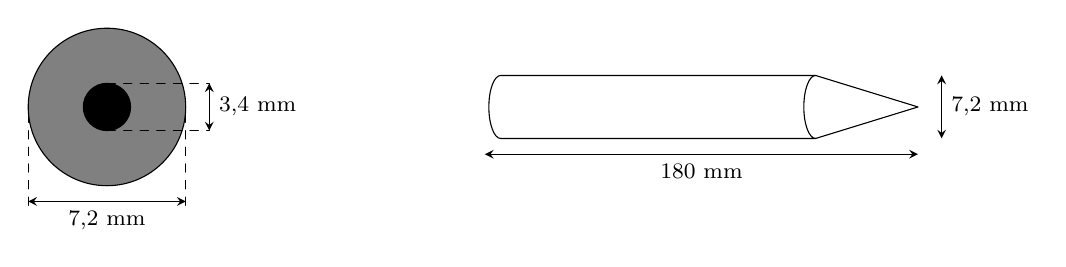
\begin{tikzpicture}[scale=1, font=\footnotesize, line join=round, line cap=round, >=stealth]
			\draw[fill=gray] (-5,0) circle (1) ;
			\draw[fill=black](-5,0) circle (0.3) ;
			\filldraw[white,draw=black] (0,0)++(90:0.4) arc (90:270:0.15 and 0.4)--++(0:4) arc (-90:-270:0.15 and 0.4)--cycle;
			\draw[dashed](-6.0,-1.25)-- (-6.0,.03);
			\draw[dashed](-4.0,-1.25)-- (-4.0,.03);
			\draw[dashed](-5,-0.3)-- (-3.7,-0.3);
			\draw[dashed](-5,0.3)-- (-3.7,0.3);
			\draw (0,0)++(0:4)++(90:0.4)--(5.3,0)--(4,-0.4);
			\draw[<->] (-3.7,-0.3) --node[midway,right]{3,4 mm} (-3.7,0.3);
			\draw[<->] (-6,-1.2) --node[midway,below]{7,2 mm} (-4,-1.2);
			\draw[<->] (-0.2,-0.6) --node[midway,below]{180 mm} (5.3,-0.6);
			\draw[<->] (5.6,0.4) --node[midway,right]{7,2 mm} (5.6,-0.4);
		\end{tikzpicture}
	\end{center}
	\begin{enumerate}
		\item Hãy tính thể tích chì cần dùng để làm lõi một cây bút chì khi chưa gọt.
		\item Để có được phần vỏ gỗ của bút chì, người ta dùng những thanh gỗ hình hộp có đáy là hình vuông cạnh $8$ mm và chiều dài $185$ mm. Hỏi với $10$ m$^3$ gỗ chuyên dụng làm vỏ bút chì thì có thể tạo ra được bao nhiêu cây bút chì, biết rằng khi xẻ nhỏ gỗ thì phần hao hụt sẽ chiếm $12\%$ do mùn cưa, gãy, gỗ lỗi, \ldots\\
		Biết công thức tính thể tích hình trụ $V=\pi R^2 h$ ($R$ là bán kính đáy, $h$ là chiều cao).
	\end{enumerate}
	\loigiai{
		\begin{enumerate}
			\item Bán kính ruột bút chì hình trụ là $R=\dfrac{3{,}4}{2} =1{,}7$ (mm).\\
			Thể tích chì cần dùng để làm lõi một cây bút chì khi chưa gọt là 
			$$V=\pi R^2 h=\pi \cdot 1{,}7^2\cdot 180 = 520{,}2\pi \approx 1\,634{,}26 \textrm{ (mm$^3$).}$$
			\item 
			Thể tích gỗ dùng để làm một vỏ bút chì là ${V_1}={8^2}\cdot 185=11\,840$ (mm$^3$).\\
			Ta có $10$ m$^3 = 10\cdot {10}^{9}$ mm$^3 = {10}^{10}$ mm$^3$.\\
			Số vỏ cây bút chì có thể làm ra được từ $10$ m$^3$ gỗ sau khi trừ đi hao hụt là
			$$\dfrac{10^{10}}{11\,840}\cdot (1-12\%) = 743\,243{,}2.$$
			Vậy với $10$ m$^3$ gỗ có thể làm được $743\,243$ vỏ bút chì thỏa mãn yêu cầu.
		\end{enumerate}
	}
\end{bt} 
\begin{bt}%[Dự án EX-9-Đề Cương Toán 9]%[Hoàng Thanh Phương]%[9H4V2-3]
	Người ta đổ một lượng nước vào một cái phễu thủy tinh. Phễu có dạng hình nón có chiều cao là $20$ cm và bán kính mặt đáy là $R$. Chiều cao của cột nước trong phễu là $10$ cm (tham khảo Hình $1$).
	\immini{
		\begin{enumerate}
			\item Tính thể tích của lượng nước trong phễu ở Hình $1$ theo $R$. Biết công thức tính thể tích $V$ của hình nón là $V=\dfrac{1}{3}\pi R^2h$, trong đó $R$ là bán kính mặt đáy, $h$ là chiều cao của hình nón.   
			\item Người ta bịt kín miệng phễu và lật ngược phễu lại (Hình 2). Chiều cao của cột nước trong phễu lúc này là bao nhiêu? (\textit{làm tròn kết quả đến hàng phần chục}).         
		\end{enumerate}
	}{
		\begin{tikzpicture}[scale=0.75, font=\footnotesize,>=stealth]%<DTools>
			\def\a{2};\def\b{0.5};\def\h{4};%Gán số liệu.
			\path %Gán tọa độ.
			(0,0) coordinate (O)
			($(O)-(0,\h)$) coordinate (S)
			($(O)-(\a,0)$) coordinate (A)
			($(O)+(\a,0)$) coordinate (B)
			($(O)-(90:\h/2)$) coordinate (S')
			($(S')+(180:\a/2)$) coordinate (A')
			($(S')+(0:\a/2)$) coordinate (B')
			;
			%Vẽ khối nón.
			\fill[cyan!30] (S)--(A')--(B') (A') arc (180:0:1 cm and 0.3 cm);
			\draw 
			(A) arc (-180:0:\a cm and \b cm) (A)--(S)--(B)
			(A') arc (-180:0:1 cm and 0.3 cm)
			(A) arc (180:0:\a cm and \b cm)
			(S) ++(-90:0.5)node[below]{Hình $1$};
			\draw[dashed] (A') arc (180:0:1 cm and 0.3 cm)
			(O)--++(180:1.3*\a) (S)--++(180:1.3*\a) (S')--++(180:0.6*\a);
			\draw[<->] (S)++(180:0.6*\a) --++(90:\h/2)node[midway,sloped,above]{$10$ cm};
			\draw[<->] (S)++(180:1.3*\a) --++(90:\h)node[midway,sloped,above]{$20$ cm};
		\end{tikzpicture}
		\begin{tikzpicture}[scale=0.75, font=\footnotesize,>=stealth]%<DTools>
			\def\a{2};\def\b{0.5};\def\h{4};%Gán số liệu.
			\path %Gán tọa độ.
			(0,0) coordinate (O)
			($(O)+(0,\h)$) coordinate (S)
			($(O)-(\a,0)$) coordinate (A)
			($(O)+(\a,0)$) coordinate (B)
			($(O)+(90:0.75)$) coordinate (S')
			($(S')+(180:1.625)$) coordinate (A')
			($(S')+(0:1.625)$) coordinate (B')
			;
			%Vẽ khối nón.
			\fill[cyan!30] (A')--(A)--(B)--(B')--cycle (A') arc (180:0:1.625 cm and \b cm) (A) arc (-180:0:\a cm and \b cm);
			\draw (A) arc (-180:0:\a cm and \b cm) (A)--(S)--(B)
			(A') arc (-180:0:1.625 cm and \b cm)
			(O) ++(-90:0.5)node[below]{Hình $2$}
			;
			\draw[dashed] (A') arc (180:0:1.625 cm and \b cm)
			(A) arc (180:0:\a cm and \b cm);
		\end{tikzpicture}
	}
	\loigiai{
		\begin{enumerate}
			\item Gọi $a$ (cm) là bán kính đáy của phần nón chứa nước ở Hình $1$.
			\immini{Áp dụng định lý Thalès, ta có $\dfrac{a}{R}=\dfrac{SS'}{SO}=\dfrac{10}{20}=\dfrac{1}{2}$ nên bán kính đáy của cột nước trong phễu ở Hình $1$ là $a = \dfrac{R}{2}$ (cm).\\			
				Thể tích của lượng nước trong phễu ở Hình $1$ là
				$$V_1=\dfrac{1}{3}\pi\left( \dfrac{R}{2}\right) ^2\cdot10=\dfrac{5}{6}\pi R^2 \text{ (cm$^3$).}$$    
			}{
				\begin{tikzpicture}[scale=0.9, font=\footnotesize,>=stealth]%<DTools>
					\def\a{2};\def\b{0.5};\def\c{0.75};\def\d{1.625};\def\h{3};%Gán số liệu.
					\path %Gán tọa độ.
					(0,0) coordinate (O)
					($(O)+(0,-\h)$) coordinate (S)
					($(O)+(-\a,0)$) coordinate (A)
					($(O)!1/2!(S)$) coordinate (S')
					($(A)!1/2!(S)$) coordinate (A')
					;
					\fill[cyan!30] (A')--(S)--(S')--(A');
					\draw (S)--(A)--node[above]{$R$}(O)--(S) (A')--node[above]{$a$}(S')--(O);
					\draw[<->] (A)++(180:0.6) --++(-90:\h)node[midway,sloped,below]{$20$ cm};
					\draw[<->] (A')++(180:0.8) --++(-90:\h/2)node[midway,sloped,below]{$10$ cm};
					\foreach \x/\g in {A/90,S/-90,O/90,A'/200,S'/0}\fill[black] (\x) circle (1.5pt)+(\g:3mm) node{$ \x $};
					\foreach \a/\b/\c in {S/O/A,S/S'/A'} {\draw pic [draw, angle radius=5pt] {right angle=\a--\b--\c};}
				\end{tikzpicture}
			}
			\item Thể tích phễu là $V=\dfrac{1}{3} \pi R^2 \cdot 20=\dfrac{20}{3} \pi R^2$ (cm$^3$).			
			\immini{Thể tích phần phễu không chứa nước ở Hình $1$ là \\
				$V_0=V-V_1=\dfrac{20}{3} \pi R^2 -\dfrac{5}{6} \pi R^2 = \dfrac{35}{6} \pi R^2$ (cm$^3$).\\
				Gọi $h$ (cm) là chiều cao của cột nước trong phễu ở Hình $2$\\ và $r$ (cm) là bán kính đáy của phần nón không chứa nước ở Hình $2$.\\
				Áp dụng định lý Thalès, ta có $\dfrac{r}{R}=\dfrac{20-h}{20}$, hay $r=\dfrac{R(20-h)}{20}$.\\
				Thể tích nón không chứa nước ở Hình 2 là
			}{
				\begin{tikzpicture}[scale=0.9, font=\footnotesize,>=stealth]%<DTools>
					\def\a{2};\def\b{0.5};\def\c{0.75};\def\d{1.625};\def\h{3};%Gán số liệu.
					\path %Gán tọa độ.
					(0,0) coordinate (O)
					($(O)+(0,\h)$) coordinate (S)
					($(O)+(\a,0)$) coordinate (A)
					($(O)!2/8!(S)$) coordinate (S')
					($(A)!2/8!(S)$) coordinate (A')
					;
					\fill[cyan!30] (A')--(A)--(O)--(S')--(A');
					\fill (A)--node[below]{$R$}(O);
					\draw (S)--(A)--(O)--(S) (A')--node[above]{$r$}(S')--node[left=-0.1cm]{$h$}(O);
					\draw[<->] (O)++(180:0.7) --++(90:\h)node[midway,sloped,above]{$20$ cm};
					\foreach \x/\g in {A/0,S/90,O/180,A'/20,S'/180}\fill[black] (\x) circle (1.5pt)+(\g:3mm) node{$ \x $};
					\foreach \a/\b/\c in {S/O/A,S/S'/A'} {\draw pic [draw, angle radius=5pt] {right angle=\a--\b--\c};}
				\end{tikzpicture}
			}
			$V_2=\dfrac{1}{3} \pi r^2(20-h)=\dfrac{1}{3} \pi\left[\dfrac{R(20-h)}{20}\right]^2(20-h)=\dfrac{1}{1\,200} \pi R^2(20-h)^3
			$ (cm$^3$).\\
			Vì thể tích phần phễu không chứa nước là không đổi nên
			\allowdisplaybreaks
			\begin{eqnarray*}
				V_0&=&V_2\\
				\dfrac{35}{6} \pi R^2&=&\dfrac{1}{1\,200} \pi R^2(20-h)^3\\
				(20-h)^3&=&7\,000\\
				20-h&=&\sqrt[3]{7\,000}\\
				h&=&20-\sqrt[3]{7\,000} \approx 0{,}9 \text{ (cm).}
			\end{eqnarray*}
			Vậy chiều cao của cột nước trong phễu lúc này là khoảng $0{,}9$ (cm).
		\end{enumerate}
	}
\end{bt}
% In đáp án trắc nghiệm
\Closesolutionfile{ans}
\indapan{6}{ans/ans-9C10-OTC}
